%%% TeX-command-extra-options: "-shell-escape"
%%%
% Created 2020-10-18 Sun 17:08
% Intended LaTeX compiler: pdflatex
\documentclass[11pt]{article}
\usepackage[utf8]{inputenc}
\usepackage[T1]{fontenc}
\usepackage{graphicx}
\usepackage{grffile}
\usepackage{longtable}
\usepackage{wrapfig}
\usepackage{rotating}
\usepackage[normalem]{ulem}
\usepackage{amsmath}
\usepackage{textcomp}
\usepackage{amssymb}
\usepackage{capt-of}
\usepackage{hyperref}
\usepackage{minted}
\IfFileExists{./resources/style.sty}{\usepackage{./resources/style}}{}
\IfFileExists{./resources/referencing.sty}{\usepackage{./resources/referencing}}{}
\addbibresource{./resources/references.bib}
\usepackage[mode=buildnew]{standalone}
\usepackage{tikz}
\usetikzlibrary{decorations.fractals}
\usetikzlibrary{lindenmayersystems}
\author{Ryan Greenup}
\date{\today}
\title{Page Rank}
\hypersetup{
 pdfauthor={Ryan Greenup},
 pdftitle={Page Rank},
 pdfkeywords={},
 pdfsubject={},
 pdfcreator={Emacs 27.1 (Org mode 9.4)}, 
 pdflang={English}}
\begin{document}

\maketitle
\tableofcontents



\section{Introduction}
\label{sec:org93e4f0c}
Any collection of interconnected information can form a network structure,
consider for example citations, webpages, wikis, power grids, wiring diagrams, encyclopedias and interpersonal
relationships. The analysis of these networks can be used to draw insights about
the behaviour of such networks.

One important form of analysis is \emph{netowork centrality}, a concept concerned with
the measure of the importance, popularity and relevance of a node. In a
relatively small graph, visualised in such a way so as to minimise the
overlapping of edges, a general expectation would be that the centrality score
would be correlated with geometric-centrality, this is demonstrated in figure
\ref{example-rs-graph} where the 2nd vertex has the highest \emph{PageRank} score and
is geometrically very central.

\subsection{The PageRank Method}
\label{sec:org9a3667e}

There are multiple ways to measure network centrality but this report is
concerned with the \emph{PageRank} method, this method asserts that the centrality of
a vertex can be measured by the frequency of traversal during a random walk.

This approach relies on the assumption tha the random walk can:

\begin{enumerate}
\item Traverse the entire network
\item Escape dead ends on a directed graph
\end{enumerate}


and so the \emph{PageRank} method involves modifying a graph in some way to adress
these assumptions, specifically by modifying the corresponding probability
transition matrix to be stochastic and primitive.

\subsection{Power Walk and the Random Surfer}
\label{sec:org109f9e7}
The typical method to adjust the transition probability matrix is the \emph{Random
Surfer}, introduced by Page and Brin in 1998
 \cite{larrypageAnatomyLargescaleHypertextual1998} as a distinguishing feature of
the \emph{Google} search engine, this aproach essentially introduces some probability
of teleporting to other nodes during a random walk, this is illustrated in
figure \ref{fig:rseg}.

A shortcoming of this approach is that it assumes all edges are positively weighted. This
menas that the model treats any link as an endorsement of the destination
node, this may not necessarily always be true (consider for exmple burned-in
advertisements or negative reviews). In the past attributing weights to links was not particularly feasible, recent developments in sentiment analysis has however made this possible meaning that this limitation is more significant.

The \emph{Power Walk} approach, introduced by Park and Simoff in 2013 \cite{parkPowerWalkRevisiting2013} is an alternative way to create a transition
probability matrix that is defined for real weighted edges and could be used with sentiment analysis to more effectively measure network centrality.

These individual approaches are discussed in more detail at \S \ref{PageRank-Generally}.

\subsection{Stability and Convergence}
\label{sec:orgcefa601}

The rate at which the algorithm for \emph{PageRank} converges to a solution and the stability of that solution can both be measured by the second eigenvalue of the corresponding transition probability matrix (The details of this are discussed at \ref{implement_models} )

It is not clear how the second eigenvalue is related to the method parameters of the \emph{Power Walk} algorithm \cite[\textsection 3.4]{parkPowerWalkRevisiting2013} and this report aims to:

\begin{enumerate}
\item Implement methods to perform \emph{PageRank} analysis using:
\begin{enumerate}
\item The \emph{Random Surfer} model
\item The \emph{Power Walk} model
\end{enumerate}
\item Investigate the Relationship between the parameters of the \emph{Power Walk}
transition probability matrix and the second eigenvalue
\end{enumerate}

\part{Implementing PageRank}
\section{Definitions use in this report}
\label{definitions}
The following definitions are used throughout this report \footnote{see generally \cite[Ch. 15]{langvilleGooglePageRankScience2012} for further reading}:

\begin{description}
\item[{Markov Chains}] are discrete mathematical model such that future values depend only on current values \cite[\textsection 1.5]{larsonElementaryLinearAlgebra1991}, this captures the concept of a random walk because the next destination depends only on the current location.
\item[{Stochastic Matrices}] contain only positive values where each column sums to 1 \cite{langvilleGooglePageRankScience2012,larsonElementaryLinearAlgebra1991} (i.e. \(\mathbf{T}\) is stochastic \(\iff \vec{1}\mathbf{T} = \vec{1}\))
\begin{itemize}
\item some authors use rows (see e.g. \cite[\textsection 15.3]{langvilleGooglePageRankScience2012}), in this paper columns will be used, i.e. columns will add to one and an entry \(\mathbf{A}_{i,j} \neq 0\) will indicate that travel is permitted from vertex \(j\) to vertex \(i\).
\begin{itemize}
\item \emph{Column Stochastic} and \emph{Row Stochastic} can be used to more clearly distinguish between which type of stochastic matrix is being used.
\end{itemize}
\item Many programming languages return \emph{unit-eigenvectors} \(\vec{x}\) such that \(\left\lvert \left\lvert \vec{x} \right\rvert \right\rvert = 1\) as opposed to \(\mathtt{sum} \left( \vec{\mathtt{x}}\right) = 1\), so when solving for a stationary vector it can be necessary to perform \(\vec{\mathtt{p}} \leftarrow \frac{\vec{\mathtt{p}}}{\sum \vec{p}}\)
\end{itemize}
\item[{Irreducible}] graphs have a path from from any given vertex to another vertex. \cite[\textsection 15.2]{langvilleGooglePageRankScience2012}
\begin{description}
\item[{Ergodic}] graphs are irreducible graphs with further constraints outside
the scope of this report (see e.g.
\cite{nathanaelackermancameronfreeralexkruckmanandrehanapatelProperlyErodicStructures2017,chenEigenvaluesInequalitiesErgodic2005})
\begin{itemize}
\item It is a necessary but not a sufficient condition of ergodic graphs that all vertices be reachable from any other vertices (see \cite{sazProbabilityTheoryThis} for a counter example.)
\end{itemize}
\end{description}
\item[{Primitive Matrices}] are non-negative irreducible matrices that have only one eigenvalue on the unit circle.
\begin{itemize}
\item If a matrix is primitive it will approach a limit under exponentiation \cite[\textsection 15.2]{langvilleGooglePageRankScience2012}, hence the significance of this concept.
\end{itemize}
\item[{Transition Probability Matrix}] is a stochastic matrix where each column is a vector of probabilities such that \(\mathbf{T}_{i,j}\) represents the probability of travelling from vertex \(j\) to vertex \(i\) during a random walk.
\begin{itemize}
\item Some Authors consider the transpose (see e.g. \cite{langvilleGooglePageRankScience2012}).
\end{itemize}
\item[{Aperiodic}] Markov chains have an irreducible and primitive transition probability matrix.
\begin{itemize}
\item If the transition probability matrix is irreducible and imprimitive it is said to be a periodic Markov chain.
\end{itemize}
\item[{Regular}] Markov Chains are irreducible and aperiodic.
\item[{Sparse}] Matrices contain a majority of elements with values equal to 0 \cite[\textsection 4.2]{langvilleGooglePageRankScience2012}
\item[{PageRank}] A process of measuring graph centrality by using a random walk algorithm and measuring the most frequent node
\begin{itemize}
\item In the literature (see e.g.
\cite{guptaWTFWhoFollow2013,langvilleGooglePageRankScience2012}) the term \emph{Random
Surfer} is usually used to refer specifically to the smoothing
algorithm shown in \eqref{eq:random-surfer}, but \emph{PageRank} refers to the entire concept including the \emph{Random Surfer}. In this report the term \emph{PageRank} is used more generally to denote the concept the model \emph{Random Surfer} or \emph{Power Walk} is denoted specifically where necessary.
\end{itemize}
\end{description}
\subsection{Notation}
\label{notation}
\begin{itemize}
\item \(\mathbf{A}\)
\begin{itemize}
\item Is the \emph{adjacency matrix} of a graph such that \(\mathbf{A}_{i,j} = 1\) indicates travel from \(j\) to \(i\) is possible.
\end{itemize}
\item \(\mathbf{T}\)
\begin{itemize}
\item Is the \emph{transition probability matrix} of a graph, this matrix indicates the probability of a movement during a random walk, such that \(\mathf{T}_{i,j}\) is equal to the probability of travelling \(j \rightarrow  i\) during a random walk.
\end{itemize}
\item \(\mathbf{D}_{\mathbf{A}}=\mathrm{diag}\left(\vec{1}\mathbf{A}\right)\)
\item \(\mathbf{D}_{\mathbf{A}}^{- 1}  =
   \begin{cases}
   0 ,& \quad \left[ \mathbf{D}_{\mathbf{A}} \right]_i = 0 \\
   \left[ \frac{1}{\mathbf{D}_{\mathbf{A}}} \right] ,& \enspace \enspace \left[ \mathbf{D}_{\mathbf{A}} \right]_i \neq 0
   \end{cases}\)
\begin{itemize}
\item A diagonal scaling matrix such that \(\mathbf{T} = \mathbf{A} \mathbf{D}_{\mathbf{A}}^{-1}\), the piecewise definition is such that \(\mathbf{D}^{-1}_{\mathbf{A}}\) is still defined even if \(\mathbf{A}\) is a reducible graph.
\begin{itemize}
\item Where \(\mathbf{D}^{-1}\) is a matrix such that multiplication with which scales each column of \(\mathbf{A}\) to 1.
\item \(\mathbf{D}^{-1}_{\mathbf{A}} = \vec{1}\mathbf{D}^{-1}_{\mathbf{A}} = \frac{1}{\vec{1}\mathbf{D}_{\mathbf{A}}}\) for some stochastic matrix \(\mathbf{A}\)
\end{itemize}
\end{itemize}
\item \(n\)
\begin{itemize}
\item Refers to the number of vertices in a graph, \(n = \mathtt{nrow}\left(\mathbf{A}\right) = \mathtt{ncol}\left(\mathbf{A}\right)\)
\end{itemize}
\item \(\mathbf{E}_{i,j} = \frac{1}{n}\)
\begin{itemize}
\item A matrix of size \(n\times n\) representing the background probability of jumping to any vertex of a graph.
\end{itemize}
\item \(\vec{1}\)
\begin{itemize}
\item a vector of length \(n\) containing only the value 1, this size of which should be clear from the context.
\begin{itemize}
\item The convention that a vector behaves as a vertical \(n \times 1\) matrix will be used here.
\item Some authors use \(\mathbf{e}\), see e.g. \cite{langvilleGooglePageRankScience2012}
\end{itemize}
\end{itemize}
\item \(\mathbf{J} = \vec{1}\cdot \vec{1}^{\mathrm{T}} \iff \mathbf{J}_{i,j} = 1\)
\begin{itemize}
\item A completely dense \(n \times n\) matrix containing only 1
\end{itemize}
\item \(\xi_{n}\)
\begin{itemize}
\item The \(n^{\mathrm{th}}\) largest eigenvalue of \(\mathbf{T}\), the use of \(\lambda\) has been avoided because some authors use \(\lambda\) to represent damping factor \(\alpha\), given that \(\alpha\)=\(\xi_{2}\) for certain graphs, this can be very ambiguous.
\end{itemize}
\item \(\alpha\)
\begin{itemize}
\item A probability such that \(\left(1-\alpha\)$\backslash$) represents of teleporting from one vertex to another during a random walk, see \ref{fig:rseg}.
\begin{itemize}
\item In the literature \(\alpha\) is often referred to as a damping factor (see e.g.  \cite{berkhoutRankingNodesGeneral2018a,brinkmeierPageRankRevisited2006a,fuDampingFactorGoogle2006,kamvarAdaptiveMethodsComputation2004b,bianchiniPageRank2005}) or a smoothing constant (see e.g \cite{koppelMeasuringDirectIndirect2014}).
\end{itemize}
\end{itemize}
\end{itemize}

\section{Mathematics of Page Rank}
\label{PageRank-Generally}
\subsection{The Stationary Distribution of a Probability Transition Matrix}
\label{stationary-distribution-of-t}
A graph can be expressed as an adjacency matrix \(\mathbf{A}\):

\[
\mathbf{A}_{i,j} \in \left\{ 0,1 \right\}
\]

Where each element of the matrix indicates whether or not travel from
vertex \(j\) to vertex \(i\) is possible with a value of 1. \footnote{Some
authors define an adjacency matrix transposed (see e.g.
\cite{rosenDiscreteMathematicsIts2007,meghabghabSearchEnginesLink2008})
this unfourtunately includes the \texttt{igraph} library
\cite{gaborcsardiIgraphManualPages2019} but that convention will not be
followed in this paper}

During a random walk on a graph the probability of arriving at vertex \(j\) from vertex
\(i\) can similarly be described as an element of a transition probability
matrix \(\mathbf{T}_{i,j}\), this matrix can be described by the following
relationship:

\begin{align}
\mathbf{T} &= \mathbf{A} \mathbf{D}^{-1}_{\mathbf{A}} \label{eq:basic-trans-def}
\end{align}

The value of \(\mathbf{D}^{-1}_{\mathbf{A}}\) is such that under matrix
multiplication \(\mathbf{A}\) will have columns that sum to 1 \footnote{such a matrix is said to be a \emph{column stochastic
matrix}, for a
reducible or non-stochastic graph the definition of
\(\mathbf{D}^{-1}_{\mathbf{A}}\) needs to piecewise, as shown in \S \ref{definitions}}, this matrix is the \emph{transition probability
matrix} \(\mathbf{T}\).

During the random walk, the running tally of frequencies, at the
\(i^{\mathrm{th}}\) step of the walk, can be described by a state distribution
vector \(\vec{p}\), this vector can be determined for each step by matrix
multiplication:

\begin{align}
\vec{p_{i+1}} = \mathbf{T}\vec{p_{i}} \label{eq:recurrence}
\end{align}

This relationship is a linear recurrence relation, more generally however it is
a \emph{Markov Chain} and \cite[\S 4.4]{langvilleGooglePageRankScience2012} and
Finding the Stationary point for this relationship will give a frequency
distribution for the nodes and a metric to measure the centrality of vertices.

\subsection{Random Surfer Model}
\label{sec:org046df67}
\subsubsection{Problems with the Stationary Distribution}
\label{issues}
The approach to measuring centrality using a stationary distrubition in \S\ref{stationary-distribution-of-t} has the following issues

\begin{enumerate}
\item Convergence of \eqref{eq:recurrence}
\begin{enumerate}
\item Will this relationship converge or diverge?
\item How quickly will it converge?
\item Will it converge uniquely?
\end{enumerate}
\item Reducible graphs
\begin{enumerate}
\item If it is not possible to perform a random walk across an entire graph for
all initial conditions the resulting frequencies of node traversal are not
meaningful.
\end{enumerate}
\item Cycles
\begin{enumerate}
\item A graph that is cyclical may not converge uniquely
\begin{enumerate}
\item Consider for example the graph \({\big (} A {\big )} \longleftrightarrow {\big (} B {\big )}\) or taking a directed edge into a closed loop.
\end{enumerate}
\end{enumerate}
\end{enumerate}

\subsubsection{Markov Chains}
\label{markov}
The relationship in \eqref{eq:recurrence} is a \emph{Markov Chain} \footnote{A \emph{Markov Chain} is
simply any process that evolves depending on it's current condition, it's
interesting to note however that the theory of \emph{Markov Chains} is not mentioned in any
of the original papers by page and brin
\cite[\textsection 4.4]{langvilleGooglePageRankScience2012}}  and it is known
that the relationship will converge to a value (this is known as the power method):

\begin{itemize}
\item for a stochastic irreducible markov chain \cite[\textsection 1.5.5]{larsonElementaryLinearAlgebra1991},
\item regardless of the initial condition of the process for an \emph{aperiodic} Markov chain \cite[\textsection 4.4]{langvilleGooglePageRankScience2012}
\end{itemize}

and so these concepts will be explored in order to address the issues with \eqref{eq:recurrence}.

\paragraph{Stochastic}
\label{stochastic}
If some vertex had a 0 outdegree the corresponding column sum for the adjacency
matrix describing that graph would also be zero and the matrix non-stochastic,
this could occur in the context of a random walk where a link to a page with no
outgoing links was followed (e.g. an image), this would be the end of the
walk.

So to ensure that \eqref{eq:recurrence} will converge, the probability transition
matrix must be made stochastic, to acheive this a uniform probability of teleporing from a dead end to any other vertex could be introduced:

\begin{align}
\mathrm{S} &= \mathrm{T}+ \frac{\vec{a} \cdot \vec{1}^{\mathrm{T}} }{n} \label{eq:nearly-random-surfer} \\
& a_{i} = \begin{cases}
    1      , &\enspace \mathrm{deg}\left( V_{i}\right) = 0  \\
    0      , &\enspace \mathrm{deg}\left( V_{i}\right) \neq 0
\end{cases}
\end{align}

This however would not be sufficient to ensure that \eqref{eq:recurrence} would converge, in addition the transition probability matrix must be made irreducible and aperiodic (i.e. primitive). \cite{langvilleGooglePageRankScience2012}

\begin{wrapfigure}{r}{0.4\textwidth}
    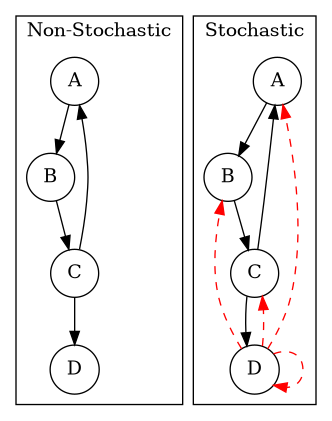
\includegraphics[width=0.38\textwidth]{media/dot/stochastic_graph_example.dot.png}

    \caption{\label{fig:stochastic-example}\(D\) is a \emph{dangling node}, a dead end during a random walk, the corresponding probability transition matrix \((\mathbf{T})\) is hence non-stochastic (and also reducible), Introducing some probability of teleporting from a dead end to any other vertex as per \eqref{eq:nearly-random-surfer} (denoted in red) will cause \(\mathbf{T}\) to be stochastic.}
\end{wrapfigure}

\paragraph{Irreducible}
\label{sec:org578c303}
A graph that allows travel from any given vertex to any other vertex is said to be irreducible \cite{langvilleGooglePageRankScience2012}, see for example figure \ref{irreducible-example}, this is important in the context of a random walk because only in an irreducible graph can all vertices be reached from any initial condition.

{
\begin{wrapfigure}{r}{0.3\textwidth}
    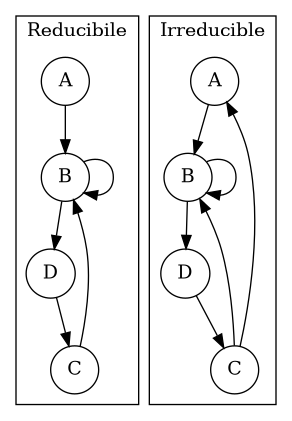
\includegraphics[width=\0.28\textwidth]{media/dot/reducible_graph_example.dot.png}

    \caption{\label{irreducible-example}Example of a reducible graph, observe that although \(C\) is not a dead end as discussed in \S \ref{stochastic}, there is no way to travel from \(C\) to \(A\), by adding an edge such an edge in the resulting graph is irreducible. The resulting graph is also aperiodic (due to the loop on \(B\)) and stochastic, so there will be a stationary distribution corresponding to \eqref{eq:recurrence}.}
\end{wrapfigure}
}

\paragraph{Aperiodic}
\label{sec:org2c6170b}
An a periodic graph has only one eigenvalue that lies on the unit circle, this is important because \(\lim_{k\rightarrow \infty} \left( \frac{\mathbf{A}}{r}^{k} \right)\) exists for a non-negative irreducible matrix \(\mathbf{A}\) if and only if \(\mathbf{A}\) is aperiodic. A graph that is a periodic can be made aperiodic by interlinking nodes \footnote{Actually it would be sufficient to merely link one vertex to itself \cite[\textsection 15.2]{langvilleGooglePageRankScience2012} but this isn't very illustrative (or helpful in this context because the graph may still be reducible or non-stochastic)}


\begin{wrapfigure}{r}{0.6\textwidth}
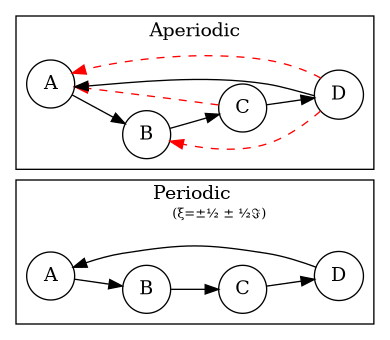
\includegraphics[width=0.55\textwidth]{media/dot/aperiodic.dot.png}
\caption{\label{fig:aperiodic}A periodic graph with all eigenvalues on the unit circle \(\xi = \frac{\sqrt{2}}{2} e^{\frac{\pi i}{4} k}\), by adding in extra edges the graph is now aperiodic (this does not represent the random surfer or power walk models, which would in theory connect every vertex with some probability)}
\end{wrapfigure}
\paragraph{The Fix}
\label{fix}
To ensure that the transition probability matrix is primitive (i.e. irreducible and aperiodic) as well as stochastic, instead of mereley introducing the possibility to teleport out of dead ends, some probability of teleporting to any node at any time can be introduced (\(1- \alpha\)), this approach is known as the \emph{Random Surfer} model and the corresponding transition probability matrix is given by \cite{larrypageAnatomyLargescaleHypertextual1998} :

\begin{align}
\mathbf{S} = \alpha \mathbf{T} + \frac{(1- \alpha)}{n} \mathbf{J} \label{eq:random-surfer}
\end{align}

This matrix is primitive and stochastic and so will converge
\cite[\textsection 4.5]{langvilleGooglePageRankScience2012}, it is also
unfourtunately completely dense, making it resource intensive to work with (see
\S \ref{solving-stationary-dist}).

Using this the relation ship in \eqref{eq:recurrence} can now be re
expressed as:

\begin{align}
\vec{p_{i+1}} \rightarrow \mathbf{S} \vec{p}_{i} \label{eq:random-surfer-recurrence}
\end{align}


{
\begin{wrapfigure}{r}{0.6\textwidth}
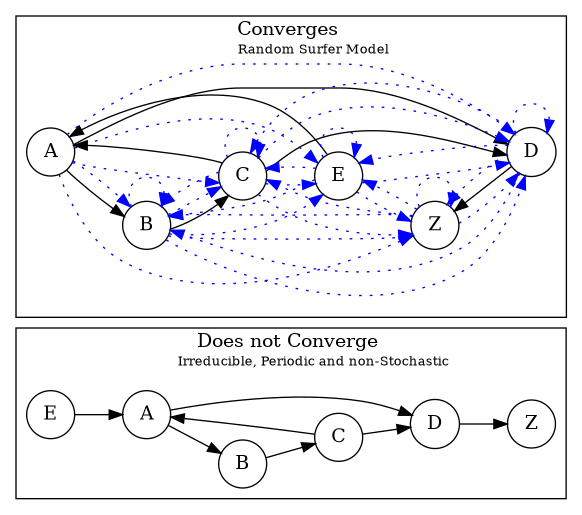
\includegraphics[width=0.6\textwidth]{media/dot/random_surfer.dot.png}
\caption{\label{fig:rseg}A graph that is aperiodic, reducible and non-stochastic, by applying the random surfer model \eqref{eq:random-surfer} blue \emph{teleportation} edges are introduced, these may be followed with a probability of \(1 - \alpha\)}
\end{wrapfigure}
}

\subsubsection{Limitations}
\label{sec:org725b0b3}
The \emph{Random Surfer} Model can only consider positively weighted edges, it cannot
take into account negatively weighted edges which might indicate that
links promote aversion rather than endorsement.
\subsection{Power walk}
\label{pwalk}
The \emph{Power Walk} method is an alternative approach to develop a probability
transition matrix to use in place of \(\mathbf{T}\) in \eqref{eq:recurrence} (and \(\mathbf{S}\) in \eqref{eq:random-surfer-recurrence}).

Let the probability of travelling to a non-adjacent vertex be some value \(x\)
and \(\beta\) be the ratio of probability between following an edge or
teleporting to another vertex.

This transition probability matrix \(\left( \mathbf{W}\right)\) would be such that the probability of
travelling to some vertex \(j \rightarrow i\) would be :

\begin{align}
\mathbf{W}_{i, j} = x\beta^{\mathbf{A_{i,j}}} \label{eq:prob-power-walk}
\end{align}

The random walk is constrained to the graph and so the probability of travelling
to one of the vertices generally is 1, hence:


\begin{align}
      1 &= \sum^{n}_{j= 1}   \left[ x \beta^{\mathbf{A_{i,j}}} \right] \\
       \implies  x&= \left( \sum^{n}_{j= 1}   \beta^{\mathbf{A_{i,j}}}
       \right)^{-1} \label{eq:powerwalk-x-val}
\end{align}

Substituting the value of \(x\) from \eqref{eq:powerwalk-x-val} into \eqref{eq:prob-power-walk} gives the probability as:

\begin{align}
      \mathbf{W}_{i,j} &= \frac{\beta^{\mathbf{A}__i,j}}{\sum^{n}_{i=j}
      \left[ \beta^{\mathbf{A}_{i,j}} \right] } \label{eq:power-walk-recurrence}
\end{align}

In this model all vertices are interconnected by some probability of jumping to
another vertex, so much like the random surfer model \eqref{eq:random-surfer} discussed
at \ref{fix} \(\mathbf{W}\) will be a primitive stochastic matrix and so if
\(\mathbf{W}\) was substituted with \(\mathbf{T}\) in \eqref{eq:recurrence} a solution
would exist.

\section{Sparse Matrices}
\label{sparse-matrix}
Most Adjacency matrices resulting from webpages and analagous networks
result in sparse adjacency matrices (see figure \ref{fig:den_undir_ba}),
this is a good thing because it requires far less computational
resources to work with a sparse matrix than a dense matrix
 \cite[\textsection 4.2]{langvilleGooglePageRankScience2012} .

Sparse matrices can be expressed in alternetive forms so as to reduce the memory
footprint associated with that matrix, one such method is \emph{Compressed Column
Storage}, this involves listing only the non-zero elements as in \eqref{eq:ordinary}
and \eqref{eq:crc}, this is implemented in \textbf{\emph{R}} with the \texttt{Matrix} package \cite{douglasbatesMatrixSparseDense2019}.

\begin{align}
    \begin{bmatrix}
	1 & 0 & 0 & 0 & 0 \\
	0 & 0 & 0 & 0 & 0 \\
	0 & \phi & 0 & 0 & 0 \\
	0 & 0 & 0 & 0 & \pi \\
	0 & 0 & 0 & 0 & 0 \\
    \end{bmatrix}  \label{eq:ordinary} \\
    \ \nonumber \\
    \ \nonumber \\
    \begin{matrix}
	\mathrm{Row\ Index} & \mathrm{Col\ Index} & \mathrm{Value}\\
	1 & 1 & 1 \\
	3 & 2 & \phi \\
	4 & 5 & \pi \\
    \end{matrix}  \label{eq:crc}
\end{align}


\subsection{Solving the Stationary Distribution}
\label{solving-stationary-dist}
The relationship in \eqref{eq:recurrence} \footnote{This assumes that the transition probability matrix \(\mathbf{T}\) is stochastic and primitive as it would be for \(\mathbf{S}\)
and \(\mathbf{W}\)} is equivelant to the eigenvalue value problem, where
\(\vec{p} = \lim_{i \rightarrow \infty} \left( \vec{p_{i}}\right)\) is the
eigenvector \footnote{More accurately the eigenvector scaled specifically to 1, so it would be more correct to say the eigenvector \(\vec{x} / \sum \vec{x}\)} \(\vec{x}\) that corresponds to the eigenvalue \(\xi=1\):

\begin{align}
\vec{p} (1) = \mathbf{S} \vec{p} \label{eq:eigenprob}
\end{align}

Solving eigenvectors for large matrices can be very resource intensive and so
this approach isn't suitable for analysing large networks, it is however an appropriate method to check against and will be implemented in this report for that purpose.

Upon iteration \eqref{eq:random-surfer-recurrence} and \eqref{eq:power-walk-recurrence} will converge to stable stationary points, as discussed
in \ref{fix}, this approach is known as the power method
\cite{larsonElementaryLinearAlgebra1991a} and is what in practice must be
implemented to solve the stationary point.

As mentioned in \S\S \ref{fix} and \ref{pwalk}, the \emph{Random Surfer} and \emph{Power Walk}
transtition probability matrices are completely dense, that means applying the
power method will not be able to take advantage of using sparse matrix
algorithms.

With some effort however it is possible to express the algorithms in such a way that only involves sparse matrices.

\section{Implementing the Models}
\label{implement_models}
To Implement the models via the power method, first they'll be implemented using
an ordinary matrix and then improved to work with sparse matrices and
algorithms, the results can be verified against \(\xi_{1}\).

The implementation has been performed with \emph{\textbf{R}} and the preamble is
provided in listing \ref{preamble}, an exemplar graph was created in listing \ref{ex-fig-r} and shown in figure \ref{example-rs-graph}, and the corresponding adjacency matrix provided in listing \ref{adj-mat-random-surf}, for the sake of comparison this graph was reproduced from \cite{parkPowerWalkRevisiting2013}.




\begin{listing}[htbp]
\begin{tcolorbox}
\begin{minted}[]{r}
  if (require("pacman")) {
      library(pacman)
    }else{
      install.packages("pacman")
      library(pacman)
    }

    pacman::p_load(tidyverse, Matrix, igraph, plotly, plot3d, mise, docstring, mise, corrplot, latex2exp)
#   options(scipen=20) # Resist Scientific Notation
\end{minted}
\caption{\label{preamble}Implemented Packages used in this report}
\end{tcolorbox}
\end{listing}


\begin{listing}[htbp]
\begin{tcolorbox}
\begin{minted}[]{r}
g1 <- igraph::graph.formula(
                1++2, 1+-8, 1+-5,
                2+-5, 2+-7, 2+-8, 2+-6, 2+-9,
                3++4, 3+-5, 3+-6, 3+-9, 3+-10,
                4+-9, 4+-10, 4+-5,
                5+-8, 6+-8, 7+-8)
plot(g1)
\end{minted}
\caption{\label{ex-fig-r}Produce exemplar graph in figure \ref{example-rs-graph}}
\end{tcolorbox}
\end{listing}


\begin{figure}{r}{0.4\textwidth}
\begin{center}
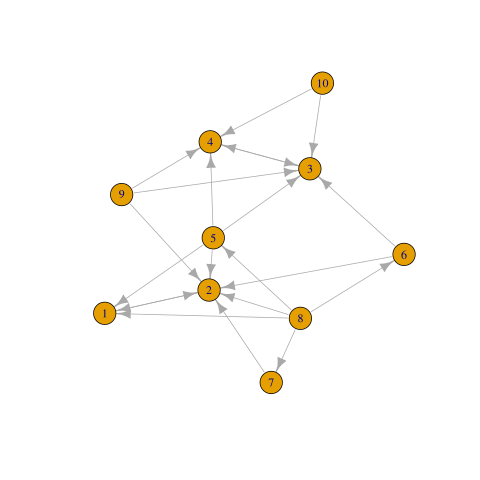
\includegraphics[width=0.28\textwidth]{media/example-graph-power-walk.png}
\end{center}
\caption{\label{example-rs-graph}Exemplar graph for \emph{PageRank} examples, produced in listing \ref{ex-fig-r}}
\end{figure}


\begin{listing}[htbp]
    \begin{tcolorbox}
        \begin{minted}[]{r}
        A <- igraph::get.adjacency(g1, names = TRUE, sparse = FALSE)

        ## igraph gives back the transpose
        (A <- t(A))
        \end{minted}
        \caption{\label{adj-mat-random-surf}Return the Adjacency Matrix corresponding to figure \ref{example-rs-graph}}
    \tcblower
        \begin{verbatim}
        1 2 8 5 7 6 9 3 4 10
        1  0 1 1 1 0 0 0 0 0  0
        2  1 0 1 1 1 1 1 0 0  0
        8  0 0 0 0 0 0 0 0 0  0
        5  0 0 1 0 0 0 0 0 0  0
        7  0 0 1 0 0 0 0 0 0  0
        6  0 0 1 0 0 0 0 0 0  0
        9  0 0 0 0 0 0 0 0 0  0
        3  0 0 0 1 0 1 1 0 1  1
        4  0 0 0 1 0 0 1 1 0  1
        10 0 0 0 0 0 0 0 0 0  0
        \end{verbatim}
    \end{tcolorbox}
\end{listing}



\subsection{Implementing the Random Surfer}
\label{sec:orgb756c9c}
\subsubsection{Ordinary Matrices}
\label{implementing-page-rank-methods}
\paragraph{Adjacency Matrix}
\label{adjacency-matrix}

\paragraph{Probability Transition Matrix}
\label{probability-transition-matrix}
The probability transition matrix is such that each column of the
initial state distribution (i.e. the transposed adjacency matrix) is
scaled to 1.

if \(\mathbf{A}\) had vertices with a 0 out-degree, the relationship in \eqref{eq:basic-trans-def} would not work, instead columns that sum to 0 would
need to be left while all other columns be divided by the column sum to get
\(\mathbf{T}\). An alternative approach using sparse matrices will be presented
below and in this case there exists corresponding \(\mathbf{T}\) that is
stochastic and so it is sufficient to use the relationship at
\eqref{eq:basic-trans-def}, this is shown in listing \ref{basic-trans-def}.

\begin{listing}[htbp]
    \begin{tcolorbox}
        \begin{minted}[]{r}
        (T <- A %*% diag(1/colSums(A)))
        \end{minted}
        \caption{\label{basic-trans-def}Solve the Transition Probability Matrix by scaling each column to 1 using matrix multiplication.}
    \tcblower
        \begin{verbatim}
        [,1] [,2] [,3] [,4] [,5] [,6]      [,7] [,8] [,9] [,10]
        1     0    1  0.2 0.25    0  0.0 0.0000000    0    0   0.0
        2     1    0  0.2 0.25    1  0.5 0.3333333    0    0   0.0
        8     0    0  0.0 0.00    0  0.0 0.0000000    0    0   0.0
        5     0    0  0.2 0.00    0  0.0 0.0000000    0    0   0.0
        7     0    0  0.2 0.00    0  0.0 0.0000000    0    0   0.0
        6     0    0  0.2 0.00    0  0.0 0.0000000    0    0   0.0
        9     0    0  0.0 0.00    0  0.0 0.0000000    0    0   0.0
        3     0    0  0.0 0.25    0  0.5 0.3333333    0    1   0.5
        4     0    0  0.0 0.25    0  0.0 0.3333333    1    0   0.5
        10    0    0  0.0 0.00    0  0.0 0.0000000    0    0   0.0
        \end{verbatim}
    \end{tcolorbox}
\end{listing}



\subparagraph{Create a Function}
\label{create-a-function}
\begin{tcolorbox}
    \begin{minted}[]{r}
    adj_to_probTrans <- function(A) {
        A %*% diag(1/colSums(A))
    }

    (T <- adj_to_probTrans(A)) %>% round(2)
    \end{minted}
\tcblower
    \begin{verbatim}
    ##    [,1] [,2] [,3] [,4] [,5] [,6] [,7] [,8] [,9] [,10]
    ## 1     0    1    0    0 0.25  0.0    0  0.2 0.00   0.0
    ## 2     1    0    0    0 0.25  0.5    1  0.2 0.33   0.0
    ## 3     0    0    0    1 0.25  0.5    0  0.0 0.33   0.5
    ## 4     0    0    1    0 0.25  0.0    0  0.0 0.33   0.5
    ## 5     0    0    0    0 0.00  0.0    0  0.2 0.00   0.0
    ## 6     0    0    0    0 0.00  0.0    0  0.2 0.00   0.0
    ## 7     0    0    0    0 0.00  0.0    0  0.2 0.00   0.0
    ## 8     0    0    0    0 0.00  0.0    0  0.0 0.00   0.0
    ## 9     0    0    0    0 0.00  0.0    0  0.0 0.00   0.0
    ## 10    0    0    0    0 0.00  0.0    0  0.0 0.00   0.0
    \end{verbatim}
\end{tcolorbox}

\paragraph{Page Rank Random Surfer}
\label{page-rank-random-surfer}
Recall from \ref{fix} the following variables of the \emph{Random Surfer} model:


\begin{align}
    \mathbf{B} &= \alpha T +  \left( 1- \alpha \right)B :\\
\ \\
    \mathbf{B}&= \begin{bmatrix}
    \frac{1}{n} & \frac{1}{n} & \ldots & \frac{1}{n} \\
    \frac{1}{n} & \frac{1}{n} & \ldots & \frac{1}{n} \\
        \vdots      & \vdots      & \ddots & \vdots  \\
    \frac{1}{n} & \frac{1}{n} & \ldots & \frac{1}{n} \\
    \end{bmatrix} \label{eq:bgval1} \\
    n&= \left| \left| V \right| \right| \\
    \alpha &\in [0,1]
\end{align}

These are
assigned to \emph{\textbf{R}} variables in listing \ref{r-var-random-surfer}.

\begin{listing}[htbp]
    \begin{tcolorbox}
        \begin{minted}[]{r}
        B <- matrix(rep(1/nrow(T), length.out = nrow(T)**2), nrow = nrow(T))
        l <- 0.8123456789

        (S <- l*T+(1-l)*B) %>% round(2)
        \end{minted}
        \caption{\label{r-var-random-surfer}Assign Random Surfer Variables, observe the unique value given to \texttt{l}, this will be relevant later.}
    \tcblower
        \begin{verbatim}
        [,1] [,2] [,3] [,4] [,5] [,6] [,7] [,8] [,9] [,10]
        1  0.02 0.83 0.18 0.22 0.02 0.02 0.02 0.02 0.02  0.02
        2  0.83 0.02 0.18 0.22 0.83 0.42 0.29 0.02 0.02  0.02
        8  0.02 0.02 0.02 0.02 0.02 0.02 0.02 0.02 0.02  0.02
        5  0.02 0.02 0.18 0.02 0.02 0.02 0.02 0.02 0.02  0.02
        7  0.02 0.02 0.18 0.02 0.02 0.02 0.02 0.02 0.02  0.02
        6  0.02 0.02 0.18 0.02 0.02 0.02 0.02 0.02 0.02  0.02
        9  0.02 0.02 0.02 0.02 0.02 0.02 0.02 0.02 0.02  0.02
        3  0.02 0.02 0.02 0.22 0.02 0.42 0.29 0.02 0.83  0.42
        4  0.02 0.02 0.02 0.22 0.02 0.02 0.29 0.83 0.02  0.42
        10 0.02 0.02 0.02 0.02 0.02 0.02 0.02 0.02 0.02  0.02
        \end{verbatim}
    \end{tcolorbox}
\end{listing}

\subparagraph{Eigen Value Method}
\label{eigen-value-method}
The eigenvector corresponding to the the eigenvalue of 1 will be the
stationary point, this is shown in listing \ref{eigenSol-rand-surf}

\begin{listing}[htbp]
    \begin{tcolorbox}
        \begin{minted}[]{r}
        print(eigen(S, symmetric = FALSE, only.values = TRUE)$values, 9)
        print(eigen(S, symmetric = FALSE)$vectors, 3)
        \end{minted}
    \tcblower
        \begin{verbatim}
        [1]  1.00000000e+00+0.0000000e+00i -8.12345679e-01+0.0000000e+00i
        [3]  8.12345679e-01+0.0000000e+00i -8.12345679e-01+0.0000000e+00i
        [5]  5.81488197e-10+0.0000000e+00i -5.81487610e-10+0.0000000e+00i
        [7] -6.74980227e-16+0.0000000e+00i  3.21036747e-17+0.0000000e+00i
        [9]  1.34928172e-18+1.1137323e-17i  1.34928172e-18-1.1137323e-17i
                [,1]         [,2]         [,3]         [,4]         [,5]
        [1,] 0.4873+0i -7.07e-01+0i  5.00e-01+0i -2.07e-03+0i -6.74e-01+0i
        [2,] 0.5268+0i  7.07e-01+0i  5.00e-01+0i  2.07e-03+0i -9.62e-02+0i
        [3,] 0.0424+0i  9.09e-18+0i -3.50e-17+0i -5.05e-17+0i  1.38e-09+0i
        [4,] 0.0493+0i -1.25e-18+0i -1.65e-16+0i  4.25e-17+0i  3.85e-01+0i
        [5,] 0.0493+0i -8.30e-18+0i -3.75e-17+0i  3.71e-17+0i  3.85e-01+0i
        [6,] 0.0493+0i -8.30e-18+0i -3.75e-17+0i  9.76e-18+0i  3.85e-01+0i
        [7,] 0.0424+0i -1.32e-18+0i -3.50e-17+0i  1.60e-17+0i -3.01e-08+0i
        [8,] 0.4915+0i -2.98e-03+0i -5.00e-01+0i -7.07e-01+0i -9.62e-02+0i
        [9,] 0.4804+0i  2.98e-03+0i -5.00e-01+0i  7.07e-01+0i -2.89e-01+0i
        [10,] 0.0424+0i  5.57e-18+0i -3.77e-17+0i  3.14e-18+0i -3.24e-08+0i
                    [,6]         [,7]         [,8]                [,9]
        [1,]  6.74e-01+0i  6.53e-01+0i -2.15e-01+0i -2.00e-01+1.53e-01i
        [2,]  9.62e-02+0i  1.09e-01+0i -1.96e-01+0i -1.59e-01+0.00e+00i
        [3,]  1.38e-09+0i  1.42e-15+0i -2.84e-16+0i -6.73e-17+1.32e-16i
        [4,] -3.85e-01+0i -4.37e-01+0i  7.85e-01+0i  6.37e-01+0.00e+00i
        [5,] -3.85e-01+0i -3.56e-01+0i  2.81e-01+0i  2.84e-02-1.63e-01i
        [6,] -3.85e-01+0i -3.58e-01+0i -3.68e-01+0i  4.84e-02-2.68e-01i
        [7,] -3.01e-08+0i -2.63e-02+0i -2.34e-01+0i -3.47e-02+4.29e-01i
        [8,]  9.62e-02+0i  1.32e-01+0i -6.40e-02+0i -1.09e-01-2.84e-01i
        [9,]  2.89e-01+0i  3.11e-01+0i  1.20e-01+0i -1.34e-01-1.50e-01i
        [10,] -3.24e-08+0i -2.82e-02+0i -1.08e-01+0i -7.64e-02+2.83e-01i
                            [,10]
        [1,] -2.00e-01-1.53e-01i
        [2,] -1.59e-01-0.00e+00i
        [3,] -6.73e-17-1.32e-16i
        [4,]  6.37e-01+0.00e+00i
        [5,]  2.84e-02+1.63e-01i
        [6,]  4.84e-02+2.68e-01i
        [7,] -3.47e-02-4.29e-01i
        [8,] -1.09e-01+2.84e-01i
        [9,] -1.34e-01+1.50e-01i
        [10,] -7.64e-02-2.83e-01i
        \end{verbatim}
    \end{tcolorbox}
\caption{\label{eigenSol-rand-surf}Solve the Eigen vectors and Eigen values of the transition probability matrix corresponding to the graph.}
\end{listing}



So in this case the stationary point corresponds to the eigenvector given by:
\[
\langle -0.49, -0.53, -0.49, -0.48, -0.05, -0.05, -0.05, -0.04, -0.04, -0.04 \rangle
\]

this can be verified by using identity \eqref{eq:eigenprob}:

$$
1 \vec{p} = S\vec{p}
$$

\begin{minted}[]{r}
  (p     <- eigen(S)$values[1] * eigen(S)$vectors[,1]) %>% Re() %>%  round(2)
\end{minted}

\begin{verbatim}
[1] 0.49 0.53 0.04 0.05 0.05 0.05 0.04 0.49 0.48 0.04
\end{verbatim}


\begin{tcolorbox}
    \begin{minted}[]{r}
        (p_new <- S %*% p) %>% Re()  %>% as.vector() %>% round(2)
    \end{minted}
 \tcblower
    \begin{verbatim}
    [1] 0.49 0.53 0.04 0.05 0.05 0.05 0.04 0.49 0.48 0.04
    \end{verbatim}
\end{tcolorbox}


However this vector does not sum to 1 so the scale should be adjusted
(for probabilities the vector should sum to 1):

\begin{tcolorbox}
    \begin{minted}[]{r}
    (p_new <- p_new/sum(p_new)) %>% Re() %>% as.vector() %>% round(2)
    \end{minted}
\tcblower
    \begin{verbatim}
    [1] 0.22 0.23 0.02 0.02 0.02 0.02 0.02 0.22 0.21 0.02
    \end{verbatim}
\end{tcolorbox}

\subparagraph{Power Value Method}
\label{power-value-method}
Using the power method should give the same result as the eigenvalue method, again but for scale:

\begin{tcolorbox}
    \begin{minted}[]{r}
    p_new <- p_new *123456789

    while (sum(round(p, 9) != round(p_new, 9))) {
        (p     <- p_new)
        (p_new <- S %*% p)
    }

    round(Re(p_new), 2) %>% as.vector()
    \end{minted}
\tcblower
    \begin{verbatim}
    [1] 26602900 28759738  2316720  2693115  2693115  2693115  2316720 26834105
    [9] 26230539  2316720
    \end{verbatim}
\end{tcolorbox}

If scaled to 1 the
same value will be returned:

\begin{tcolorbox}
    \begin{minted}[]{r}
    (p_new <- p_new/sum(p_new)) %>% Re %>% as.vector() %>% round(2)
    \end{minted}
\tcblower
    \begin{verbatim}
    [1] 0.22 0.23 0.02 0.02 0.02 0.02 0.02 0.22 0.21 0.02
    \end{verbatim}
\end{tcolorbox}
\subparagraph{Scaling}
\label{scaling}
If the initial state sums to 1, then the scale of the stationary
vector will also sum to 1, so this isn't in practice an issue for the power method:

\begin{tcolorbox}
    \begin{minted}[]{r}
    p     <- c(1, 0, 0, 0, 0, 0, 0, 0, 0, 0)
    p_new <- S %*% p

    while (sum(round(p, 9) != round(p_new, 9))) {
        (p     <- p_new)
        (p_new <- S %*% p)
    }

    cbind(p_new, p)
    \end{minted}
\tcblower
    \begin{verbatim}
            [,1]       [,2]
    1  0.21548349 0.21548349
    2  0.23295388 0.23295388
    8  0.01876543 0.01876543
    5  0.02181424 0.02181424
    7  0.02181424 0.02181424
    6  0.02181424 0.02181424
    9  0.01876543 0.01876543
    3  0.21735625 0.21735625
    4  0.21246737 0.21246737
    10 0.01876543 0.01876543
    \end{verbatim}
\end{tcolorbox}

\subsubsection{Sparse Matrices}
\label{sec:org1aa2d1c}
\paragraph{Creating the Probability Transition Matrix}
\label{sec:org04def23}
Implementing the page rank method on a larger graph requires the use of more
efficient form of matrix storage as discussed at \ref{sparse-matrix}

A sparse matrix can be created using the following syntax, which will return a
matrix of the class \texttt{dgCMatrix}:

\begin{tcolorbox}
    \begin{minted}[]{r}
    library(Matrix)
    ## Create Example Matrix
    n <- 20
    m <- 10^6
    i <- sample(1:m, size = n); j <- sample(1:m, size = n); x <- rpois(n, lambda = 90)
    A <- sparseMatrix(i, j, x = x, dims = c(m, m))

    summary(A)
    \end{minted}
\tcblower
    \begin{verbatim}
    1000000 x 1000000 sparse Matrix of class "dgCMatrix", with 20 entries
            i      j   x
    1  141572  65888  92
    2  547799  69135  87
    3  368656 123865  87
    4  881320 129763 111
    5   53637 154979  92
    6  193808 192238 100
    7  467415 260074  86
    8   28105 276311  79
    9  481097 316591 102
    10 559159 319674  93
    11 927895 322174  77
    12 562619 372818  82
    13 123000 391022  80
    14  75909 417462  70
    15 309593 457917  78
    16 434992 521070 101
    17 617821 769436  93
    18 673173 811478 103
    19 860284 841473 104
    20 734100 852938  83
    \end{verbatim}
\end{tcolorbox}

As before in section \ref{probability-transition-matrix}, the probability transition matrix can be found by:

\begin{enumerate}
\item Creating adjacency matrix
\begin{enumerate}
\item Transposing as necessary such that \(\mathbf{A}_{i,j}\neq 0\) indicates that \(j\) is connected to \(i\) by a directed edge.
\end{enumerate}
\item Scaling the columns to one
\end{enumerate}

To implement this for a sparseMatrix of the class \texttt{dgCMatrix}, the same
technique of multiplying by a diagonalised matrix as in \eqref{eq:diagScaleDef} may be
implemented, using sparse matrices has the advantage however that only non-zero
elements will be operated on, meaning that columns that some to zero can still
be used to create a probability transition matrix \footnote{Although this matrix may
still have columns that sum to zero and will hence be non-stochastic}
pracice an error however to create this new matrix, a new \texttt{sparseMatrix} will
need to be created using the properties of the original matrix, this can be done
like so:

\begin{listing}[htbp]
    \begin{minted}[]{r}
    sparse_diag <- function(mat) {

    ## Get the Dimensions
    n <- nrow(mat)

    ## Make a Diagonal Matrix of Column Sums
    D <- sparseMatrix(i = 1:n, j = 1:n, x = colSums(mat), dims = c(n,n))

    ## Throw away explicit Zeroes
    D <- drop0(D)

    ## Inverse the Values
    D@x <- 1/D@x

    ## Return the Diagonal Matrix
    return(D)
    }
    \end{minted}
\caption{\label{sparse-diag}A function that takes in a column \(\rightarrow\) row adjacency matrix (\(\mathbf{A}\)) and returns a diagonal matrix (\(\mathbf{D}^{-1}_{\mathbf{A}}}\)) such that \(\vec{1}\mathbf{A} \mathbf{D}^{-1}_{\mathbf{A}} = \vec{1}\)}
\end{listing}

Applying this to the previously created sparse matrix:

\begin{minted}[]{r}
D <- sparse_diag(t(A))
summary(D)
\end{minted}

\begin{verbatim}
1000000 x 1000000 sparse Matrix of class "dgCMatrix", with 20 entries
        i      j           x
1   28105  28105 0.012658228
2   53637  53637 0.010869565
3   75909  75909 0.014285714
4  123000 123000 0.012500000
5  141572 141572 0.010869565
6  193808 193808 0.010000000
7  309593 309593 0.012820513
8  368656 368656 0.011494253
9  434992 434992 0.009900990
10 467415 467415 0.011627907
11 481097 481097 0.009803922
12 547799 547799 0.011494253
13 559159 559159 0.010752688
14 562619 562619 0.012195122
15 617821 617821 0.010752688
16 673173 673173 0.009708738
17 734100 734100 0.012048193
18 860284 860284 0.009615385
19 881320 881320 0.009009009
20 927895 927895 0.012987013
\end{verbatim}

and hence the probability transition matrix may be implemented by performing matrix multiplication accordingly:

\begin{minted}[]{r}
summary((T <- t(A) %*% D))
\end{minted}

\begin{verbatim}
1000000 x 1000000 sparse Matrix of class "dgCMatrix", with 20 entries
        i      j x
1  276311  28105 1
2  154979  53637 1
3  417462  75909 1
4  391022 123000 1
5   65888 141572 1
6  192238 193808 1
7  457917 309593 1
8  123865 368656 1
9  521070 434992 1
10 260074 467415 1
11 316591 481097 1
12  69135 547799 1
13 319674 559159 1
14 372818 562619 1
15 769436 617821 1
16 811478 673173 1
17 852938 734100 1
18 841473 860284 1
19 129763 881320 1
20 322174 927895 1
\end{verbatim}

\paragraph{Solving the Random Surfer via the Power Method}
\label{random-surfer-sparse-fix}
Solving the eigenvalues for such a large matrix will not feasible, instead the power method will need to be used to find the stationary point.

However, creating a matrix of background probabilites (denoted by \texttt{B} in section \ref{page-rank-random-surfer}) will not be feasible, it would simply be too large, instead some algebra can be used to reduce \(B\) from a matrix into a vector containing only \(\frac{1-\alpha}{N}\).

The power method is given by:

\begin{align}
\vec{p}= \mathbf{S} \vec{p}
\end{align}

where:

\begin{align}
S &= \alpha \mathbf{T} +  \left( 1 - \alpha \right) \mathbf{B} \\
\vec{p} &= \left( \alpha \mathbf{T} +  \left( 1 - \alpha \right) \mathbf{B} \right) \vec{p}\\
&= \alpha \mathbf{T}\vec{p} +  \left( 1-\alpha \right) \mathbf{B} \vec{p}
\end{align}

Let \(\mathbf{F}= \mathbf{B}\vec{p}\), consider the value of \(\mathbf{F}\) :

\begin{align}
\mathbf{F} &=
\begin{bmatrix}
\frac{1}{N} & \frac{1}{N} & \ldots & \frac{1}{N} \\
\frac{1}{N} & \frac{1}{N} & \ldots & \frac{1}{N} \\
\vdots      & \vdots      & \ddots & \vdots \\
\frac{1}{N} & \frac{1}{N} & \ldots & \frac{1}{N} \\
\end{bmatrix} \label{eq:bgVal2}
\begin{bmatrix}
\vec{p_1} \\ \vec{p_2} \\ \vdots \\ \vec{p_m}
\end{bmatrix}  \\
&= \begin{bmatrix}
\left( \sum^{m}_{i= 0}   \left[ p_i \right]  \right) \times \frac{1}{N} \\
\left( \sum^{m}_{i= 0}   \left[ p_i \right]  \right) \times \frac{1}{N} \\
\vdots  \\
\left( \sum^{m}_{i= 0}   \left[ p_i \right]  \right) \times \frac{1}{N} \\
\end{bmatrix}  \\
& \text{Probabilities sum to 1 and hence:} \\
&= \begin{bmatrix}
\frac{1}{N} \\
\frac{1}{N} \\
\frac{1}{N} \\
\vdots  \\
\frac{1}{N} \\
\end{bmatrix}
\end{align}
So instead the power method can be implemented by performing an algorithm that involves only sparse matrices:

\begin{minted}[]{r}
## Find Stationary point of random surfer
N     <- nrow(A)
alpha <- 0.85
F     <- rep((1-alpha)/N, nrow(A))  ## A nx1 vector of (1-alpha)/N

## Solve using the power method
p     <- rep(0, length.out = ncol(T)); p[1] <- 1
p_new <- alpha*T %*% p + F

## use a Counter to debug
i <- 0
while (sum(round(p, 9) != round(p_new, 9))) {
    p     <- p_new
    p_new <- alpha*T %*% p + F
    (i <- i+1) %>% print()
}

p %>% head() %>% print()
\end{minted}

\begin{verbatim}
[1] 1
[1] 2
6 x 1 Matrix of class "dgeMatrix"
        [,1]
[1,] 1.5e-07
[2,] 1.5e-07
[3,] 1.5e-07
[4,] 1.5e-07
[5,] 1.5e-07
[6,] 1.5e-07
\end{verbatim}

\subsection{Power Walk Method}
\label{sec:org97c1330}
Recall from \ref{pwalk} that the power walk is given by:

\begin{align*}
\mathbf{T} &= \mathbf{B} \mathbf{D}^{-1}_{B}
\end{align*}
\subsubsection{Ordinary Matrices}
\label{sec:org3f6b537}
Implementing the Power walk using ordinary matrices is very similar to the \emph{Random Surfer} model be done pretty much the same as it is with the random surfer, but doing it with Sparse Matrices is a bit trickier.

Create the Adjacency Matrix
\begin{minted}[]{r}
  A <- igraph::get.adjacency(g1, names = TRUE, sparse = FALSE)

## * Function to create Prob Trans Mat
adj_to_probTrans <- function(A, beta) {
    B     <- A
    B     <- beta^A           # Element Wise exponentiation
    D     <- diag(colSums(B)) # B is completely dense so D ≄ 0
    D_in  <- solve(D)         # Solve returns inverse of matrix
    W     <- B %*% D_in

    return(as.matrix(W))
}

beta <- β <- 0.867
(W <- adj_to_probTrans(A, beta = β)) %>% round(2)
\end{minted}

\begin{verbatim}
   [,1] [,2] [,3] [,4] [,5] [,6] [,7] [,8] [,9] [,10]
1  0.10 0.09  0.1 0.10 0.10 0.10  0.1 0.11 0.11   0.1
2  0.09 0.11  0.1 0.10 0.10 0.10  0.1 0.11 0.11   0.1
8  0.09 0.09  0.1 0.09 0.09 0.09  0.1 0.11 0.11   0.1
5  0.09 0.09  0.1 0.10 0.10 0.10  0.1 0.09 0.09   0.1
7  0.10 0.09  0.1 0.10 0.10 0.10  0.1 0.11 0.11   0.1
6  0.10 0.09  0.1 0.10 0.10 0.10  0.1 0.09 0.11   0.1
9  0.10 0.09  0.1 0.10 0.10 0.10  0.1 0.09 0.09   0.1
3  0.10 0.11  0.1 0.10 0.10 0.10  0.1 0.11 0.09   0.1
4  0.10 0.11  0.1 0.10 0.10 0.10  0.1 0.09 0.11   0.1
10 0.10 0.11  0.1 0.10 0.10 0.10  0.1 0.09 0.09   0.1
\end{verbatim}

Look at the Eigenvalues:
\begin{minted}[]{r}
eigen(W, only.values = TRUE)$values %>% round(9)
eigen(W)$vectors/sum(eigen(W)$vectors)
\end{minted}

\begin{verbatim}
 [1]  1.000000000+0.000000000i  0.014269902+0.000000000i
 [3] -0.014148391+0.000000000i  0.014147087+0.000000000i
 [5]  0.007672842+0.004095136i  0.007672842-0.004095136i
 [7]  0.000000000+0.000000000i  0.000000000+0.000000000i
 [9]  0.000000000+0.000000000i  0.000000000+0.000000000i
               [,1]             [,2]            [,3]            [,4]
 [1,] 0.10153165+0i  5.107247e-02+0i  0.073531664+0i  0.009918277+0i
 [2,] 0.10159353+0i -1.161249e-01+0i  0.071987451+0i -0.009531974+0i
 [3,] 0.09609664+0i -2.162636e-01+0i  0.198568750+0i  0.141245296+0i
 [4,] 0.09725145+0i  6.794340e-02+0i -0.012230606+0i -0.001148014+0i
 [5,] 0.10153165+0i  5.107247e-02+0i  0.073531664+0i  0.009918277+0i
 [6,] 0.10008449+0i  1.115133e-01+0i -0.005625969+0i -0.156796770+0i
 [7,] 0.09865794+0i  1.175228e-01+0i -0.084225633+0i  0.008563891+0i
 [8,] 0.10157348+0i -6.053608e-02+0i -0.078607240+0i  0.165540590+0i
 [9,] 0.10155286+0i -6.104664e-03+0i -0.079165209+0i -0.166535117+0i
[10,] 0.10012631+0i -9.522175e-05+0i -0.157764873+0i -0.001174456+0i
                         [,5]                    [,6]             [,7]
 [1,]  0.00633946+0.04208220i  0.00633946-0.04208220i  3.014602e-16+0i
 [2,]  0.00757768+0.03910216i  0.00757768-0.03910216i  1.909248e-16+0i
 [3,]  0.22697603+0.00000000i  0.22697603+0.00000000i  3.985744e-02+0i
 [4,] -0.11628681-0.11808928i -0.11628681+0.11808928i -2.471407e-01+0i
 [5,]  0.00633946+0.04208220i  0.00633946-0.04208220i  7.520823e-02+0i
 [6,] -0.03494625-0.01031801i -0.03494625+0.01031801i  1.719325e-01+0i
 [7,] -0.07581902-0.06371153i -0.07581902+0.06371153i  6.131013e-03+0i
 [8,]  0.00717270+0.04008639i  0.00717270-0.04008639i  5.526770e-17+0i
 [9,]  0.00675977+0.04107970i  0.00675977-0.04107970i  1.105354e-16+0i
[10,] -0.03411300-0.01231382i -0.03411300+0.01231382i -4.598845e-02+0i
                  [,8]             [,9]            [,10]
 [1,] -1.791605e-17+0i -4.365749e-17+0i  1.179767e-17+0i
 [2,] -7.334385e-17+0i -8.731498e-17+0i -5.190977e-17+0i
 [3,] -1.241234e-01+0i -1.401965e-01+0i -8.894098e-02+0i
 [4,]  1.691000e-01+0i  1.687523e-01+0i  1.041947e-01+0i
 [5,] -2.144546e-01+0i  2.715852e-02+0i  3.085359e-02+0i
 [6,]  4.535455e-02+0i -1.959109e-01+0i -1.350483e-01+0i
 [7,]  7.398187e-02+0i  3.163948e-02+0i -1.260060e-01+0i
 [8,]  8.062225e-17+0i  3.638124e-17+0i  5.898837e-18+0i
 [9,]  2.687408e-17+0i  3.638124e-17+0i  5.662884e-17+0i
[10,]  5.014155e-02+0i  1.085570e-01+0i  2.149470e-01+0i
\end{verbatim}

Unlike the \emph{Random Surfer} Model in listing \ref{eigenSol-rand-surf} at \ref{eigen-value-method} the relationship between the second eigenvalue and the model parameters is not as clear, this provides that the

Use the power method

\begin{minted}[]{r}
## * Power Method
p    <- rep(0, nrow(W))
p[1] <- 1
p_new    <- rep(0, nrow(W))
p_new[2]    <- 1

while (sum(round(p, 9) != round(p_new, 9))) {
    (p     <- p_new)
    (p_new <- W %*% p)
}


p %>% as.vector()
\end{minted}

\begin{verbatim}
[1] 0.10153165 0.10159353 0.09609664 0.09725145 0.10153165 0.10008449
[7] 0.09865794 0.10157348 0.10155286 0.10012631
\end{verbatim}

\subsubsection{Sparse Matrices}
\label{sec:org5192cbb}
\paragraph{Theory; Simplifying Power Walk to be solved with Sparse Matrices}
\label{sec:org82fb181}
The Random Surfer model is:

$$\begin{aligned}
    \mathbf{S} &= \alpha \mathbf{T} +  \mathbf{F}  \label{eq:sparse-RS}\end{aligned}$$

where:

\begin{itemize}
\item \(\mathbf{T}\)

\begin{itemize}
\item is an \(i \times j\) matrix that describes the probability of
travelling from vertex \(j\) to \(i\)

\begin{itemize}
\item This is transpose from the way that \texttt{igraph} produces an adjacency
matrix.
\end{itemize}
\end{itemize}

\item \(\mathbf{F} = \begin{bmatrix} \frac{1}{n} \\ \frac{1}{n} \\ \frac{1}{n} \vdots \end{bmatrix}\)
\end{itemize}

Interpreting the transition probability matrix in this way is such that
\(\mathbf{T}= \mathbf{A}\mathbf{D}^{- 1}_A\) under the following
conditions:


\begin{itemize}
\item No column of \(\mathbf{A}\) sums to zero

\begin{itemize}
\item If this does happen the question arises how to deal with
\(\mathbf{D_\mathbf{A}^{- 1}}\)

\begin{itemize}
\item I've been doing \(\mathbf{D}^{\mathrm{T}}_{\mathbf{A}, i, j} := \mathtt{diag} \left( {\frac{1}{\mathtt{colsums}\left( \mathbf{A} \right)}} \right)\)
and then replacing any \(0\) on the diagonal with 1.
\end{itemize}

\item What is done in the paper is to make another matrix \(\mathbf{Z}\)
that is filled with 0, if a column sum of \(\mathbf{A}\) adds to zero
then that column in \(\mathbf{Z}\) becomes \(\frac{1}{n}\)

\begin{itemize}
\item This has the effect of making each row identical

\item The probability of going from an orphaned vertex to any other
vertex would hence be \(\frac{1}{n}\)

\item The idea with this method is then to use
\(D_\mathbf{\left( A+Z \right)}^{- 1}\) this will be consistent with
the \emph{Random Surfer} the method using \(\mathbf{F}\) in
[[\#eq:sparse-RS][]] \eqref{eq:sparse-RS}
\end{itemize}

where each row is identical that is a 0
\end{itemize}
\end{itemize}

The way to deal with the \emph{Power Walk} is more or less the same.

observe that:

\begin{align}
   \left( \mathbf{B} = \beta^{\mathbf{A}} \right)\wedge \left( \mathbf{A}_{i, j}\right)\in \mathbb{R}  \implies  \left\lvert \mathbf{B}_{i, j} \right\rvert > 0 \quad \forall i,j>n\in \mathbb{Z}^+ \label{eq:b-is-pos}
\end{align}



Be mindful that the use of exponentiation in \eqref{eq:b-is-pos} is not an element wise
exponentiation and not an actual matrix exponential.

So if I have:

\begin{itemize}
\item \(\mathbf{O}_{i, j} := 0, \quad \forall i,j\leq n \in \mathbb{Z}^+\)

\item \(\vec{p_i}\) as the state distribution, being a vector of length \(n\)
\end{itemize}

Then It can be shown (see \eqref{eq:sparse-power-walk} at \ref{solve-background-prob-power-walk-sparse}):

\begin{align}
    \mathbf{O} \mathbf{D}_{\mathbf{B}}^{-1} \vec{p_i} &= (\overrightarrow{\delta^{{\footnotesize \tmmathbf{T}}}}
     \overrightarrow{p_i})  \vec{1}\\
& = \mathtt{repeat} \left(\vec{p} \bullet \vec{\delta^{\tiny \mathrm{T}}} \mathtt{, n} \right) \\
\end{align}



where:

\begin{itemize}
\item \(\vec{\delta_i} = \frac{1}{\mathtt{colsums} \left( \mathbf{B} \right)}\)
\begin{itemize}
\item A vector\ldots{}(\(n\times 1\) matrix)
\end{itemize}
\item[{\(\vec{1}\) }] is a vector containing all 1's
\begin{itemize}
\item A vector\ldots{}(\(n\times 1\) matrix)
\end{itemize}
\item[{\(\vec{\delta^{\mathrm{T}}}\)}] refers to the transpoxe of \(\vec{\detla}\) (\(1\times n\) matrix)
\item[{\(\vec{\delta^{\mathrm{T}}} \vec{p_{i}}\)}] is some number (because it's a dot product)
\end{itemize}

This means we can do:

\begin{align}
  \overrightarrow{p_{i + 1}} & = \mathbf{T}_{\mathrm{pw}}
  \overrightarrow{p_i}\\
& = \mathbf{BD}_{\mathbf{B}}^{- 1}
  \overrightarrow{p_i}\\
  & = \left( \mathbf{B} - \mathbf{O} + \mathbf{O} \right)
  \mathbf{D}_{\mathbf{B}}^{- 1} \overrightarrow{p_i}\\
  & = \left( \left( \mathbf{B} - \mathbf{O} \right)
  \mathbf{D}_{\mathbf{B}}^{- 1} + \mathbf{OD}_{\mathbf{B}}^{- 1} \right)
  \overrightarrow{p_i}\\
  & = \left( \mathbf{B} - \mathbf{O} \right) \mathbf{D}_{\mathbf{B}}^{- 1}
  \overrightarrow{p_i} + \mathbf{OD}_{\mathbf{B}}^{- 1} \overrightarrow{p_i}\\
  & = \left( \mathbf{B} - \mathbf{O} \right) \mathbf{D}_{\mathbf{B}}^{- 1}
  \overrightarrow{p_i} + \vec{1} (\overrightarrow{\delta^{\mathrm{T}}}
  \overrightarrow{p_i}) \\
  & = \left( \mathbf{B} - \mathbf{O} \right) \mathbf{D}_{\mathbf{B}}^{- 1}
  \overrightarrow{p_i} + \mathtt{rep} (\overrightarrow{\delta^{\mathrm{T}}}
  \overrightarrow{p_i})
\end{align}

where:


Let \((\mathbf{B}-\mathbf{O}) = \mathbf{B_{\mathbf{O}}}\):

\begin{eqnarray*}
  \overrightarrow{p_{i + 1}} & = \mathbf{B_{\mathbf{O}}} \mathbf{D}_{\mathbf{B}}^{- 1}
  \overrightarrow{p_i} + \mathtt{rep} (\overrightarrow{\delta^{\mathrm{T}}}
  \overrightarrow{p_i}) &
\end{eqnarray*}

Now solve \(\tmmathbf{D}_B^{- 1}\) in terms of \(\mathbf{B_{O}}\) :

\begin{align}
  \mathbf{B}_{\mathbf{\mathbf{O}}} = & (\mathbf{B}-\mathbf{O})\\
  \mathbf{B} = & \mathbf{B}_{\mathbf{\mathbf{O}}}
  +\mathbf{O}
\end{align}

If we have \(\delta_{\mathbf{B}}\) as the column sums of\(\tmmathbf{\Beta}\) \(\mathbf{B}\):

\begin{align}
\delta^{-1}_{\mathbf{B}} &= \vec{1}\mathbf{B} \\
&= \vec{1} \left( \mathbf{B_{O}} + \mathbf{O}\right) \\
&= \vec{1}  \mathbf{B_{O}} + \vec{1}\mathbf{O} \\
&= \vec{1} \mathbf{B_{\mathbf{O}}} + \langle n, n, n, ... n \rangle \\
&= \vec{1} \mathbf{B_{\mathbf{O}}} + \vec{1} n \\
\delta_{\mathbf{B}}&=\mathtt{1/(colSums(\mathbf{B_{O}}) + n )}
\end{align}

Then if we have \(\mathit{{\tmstrong{{\tmem{D}}}}}_{\mathit{{\tmem{{\tmstrong{B}}}}}} =
\mathtt{diag} (\delta_{\tmmathbf{B}}) \mathtt{}\):


\[ \begin{array}{lll}
     \mathit{{\tmstrong{{\tmem{D}}}}}_{\mathit{{\tmem{{\tmstrong{B}}}}}}^{- 1}
     & = & \mathrm{diag} \left( \delta^{- 1}_{\mathbf{B}} \right)\\
     & = & \mathtt{diag} \left( \mathtt{ColSums}
     (\mathtt{\tmmathbf{B}_{\tmmathbf{O}}}) + \mathtt{n}
     \right)^{\mathtt{- 1}}
   \end{array} \]

And so the the power method can be implemented using sparse matrices:

\begin{align}
\vec{p_{i+1}} = \mathrm{B_{O}} \enspace \mathrm{diag}\left( \vec{1} \mathbf{B_{O}} + \vec{1}n \right) \vec{p_{i}} + \vec{1} \vec{\delta^{\mathrm{T}}\vec{p_{i}}}
\end{align}

in terms of \textbf{\emph{R}}:

\begin{minted}[]{r}
p_new <- Bo %*% diag(colSums(B)+n) %*% p + rep(t(δ) %*% p, n)

# It would also be possible to sum the element-wise product
(t(δ) %*% p) == sum(δ * p)

# Because R treats vectors the same as a nX1 matrix we could also
# perform the dot product of the two vectors, meaning the following
# would be true in R but not true generally

(t(δ) %*% p) == (δ %*% p)
\end{minted}


\subparagraph{Solving the Background Probability}
\label{solve-background-prob-power-walk-sparse}
In this case a vertical single column matrix will represent a vector and \(\otimes\) will represent the outer product (i.e. the \emph{Kronecker Product}):



Define \(\vec{\delta}\) as the column sums of
\[\begin{aligned}
     \vec{\delta} & = \mathtt{colsum} (\text{{\bfseries{B}}})^{- 1}\\
     & = \frac{1}{\overrightarrow{1^{{\scriptsize \ensuremath{\boldsymbol{T}}}}}
     \ensuremath{\boldsymbol{B}}}
   \end{aligned}\]


Then we have:


\[ \begin{aligned}
     \mathbf{OD}_{\mathbf{B}}^{- 1} \overrightarrow{p_i} & = \left(
     \begin{array}{cccc}
       1 & 1 & 1 & \\
       1 & 1 & 1 & \ldots\\
       1 & 1 & 1 & \\
       & \vdots &  & \ddots
     \end{array} \right) \left( \begin{array}{cccc}
       \frac{1}{\delta_1} & 0 & 0 & \\
       0 & \frac{1}{\delta_2} & 0 & \ldots\\
       0 & 0 & \frac{1}{\delta_{13}} & \\
       & \vdots &  & \ddots
     \end{array} \right) \left( \begin{array}{c}
       p_{i, 1}\\
       p_{i, 2}\\
       p_{i, 3}\\
       \vdots
     \end{array} \right) \nonumber \nonumber\\
     & = \left( \begin{array}{cccccc}
       \frac{p_{i, 1}}{\delta 1} & + & \frac{p_{i, 2}}{\delta_2} & + &
       \frac{p_{i, 3}}{\delta_3} & \\
       \frac{p_{i, 1}}{\delta 1} & + & \frac{p_{i, 2}}{\delta_2} & + &
       \frac{p_{i, 3}}{\delta_3} & \ldots\\
       \frac{p_{i, 1}}{\delta 1} & + & \frac{p_{i, 2}}{\delta_2} & + &
       \frac{p_{i, 3}}{\delta_3} & \\
       &  & \vdots &  &  & \ddots
     \end{array} \right) \nonumber \nonumber\\
     & = \left( \begin{array}{c}
       \sum^n_{k = 1} [p_{i, k} \delta_i]\\
       \sum^n_{k = 1} [p_{i, k} \delta_i]\\
       \sum^n_{k = 1} [p_{i, k} \delta_i]\\
       \vdots
     \end{array} \right) \nonumber\\
     & = \left( \begin{array}{c}
       \overrightarrow{\delta^{{\footnotesize \tmmathbf{T}}}}
       \overrightarrow{p_i}\\
       \overrightarrow{\delta^{{\footnotesize \tmmathbf{T}}}} \vec{p}_i\\
       \overrightarrow{\delta^{{\footnotesize \tmmathbf{T}}}} \vec{p}_i\\
       \vdots
     \end{array} \right) \nonumber\\
     & = \overrightarrow{\delta^{{\footnotesize \tmmathbf{T}}}}
     \overrightarrow{p_i} \left( \begin{array}{c}
       1\\
       1\\
       1\\
       \vdots
     \end{array} \right) \nonumber\\
     & = (\overrightarrow{\delta^{{\footnotesize \tmmathbf{T}}}}
     \overrightarrow{p_i})  \vec{1}\\
     & = \mathtt{repeat} (\overrightarrow{\delta} \overrightarrow{p_i}
     \mathtt{, n}) \label{eq:sparse-power-walk}
   \end{aligned} \]
Observe also that If we let \(\vec{\delta}\) and \(p_i\) be 1 dimensional
vectors, this can also be expressed as a dot product:

\begin{center}
\begin{tabular}{ll}
Matrices & Vectors\\
\(\vec{\delta^{\mathrm{T}}} \vec{p_{i}}\) & \(\vec{\delta} \vec{p_{i}}\)\\
\end{tabular}

\end{center}

\paragraph{Practical; Implementing the Power Walk on Sparse Matrices}
\label{sec:org3a8ba15}
\subparagraph{Inspect the newly created matrix and create constants}
\label{sec:org6f79a11}
\subparagraph{Setup}
\label{sec:org19fbb8e}
\begin{enumerate}
\item Define function to create DiagonalsSparse Diagonal Function
\label{sec:org74d4373}

Unlike the Random Surfer model the diagonal scaling matrix will always be given by  \(\mathbf{D}_{B}^{-1} = \mathbf{B} \enspace \mathrm{diag}\left( \frac{1}{\vec{1}\mathbf{B}}\right)\) because \(\beta^{\mathbf{A}_{i,j}} \neq 0 \quad \forall \mathbf{A}_{i,j}\), this is convenient but in any case the \texttt{sparse\_diag} function in listing \ref{sparse-diag} will still work.
\end{enumerate}

\subparagraph{Power Walk}
\label{sec:org4e03252}
\begin{enumerate}
\item Define B
\label{sec:orgde2e7a6}
\begin{minted}[]{r}
A      <- Matrix::Matrix(A, sparse = TRUE)
B      <- A
B@x    <- β^(A@x)
B      <- A
B       <- β^A

Bo     <- A

# These two approaches are equivalent
Bo@x   <- β^(A@x) -1   # This in theory would be faster
# Bo     <- β^(A) -1
# Bo     <- drop0(Bo)


 n <- nrow(A)
\end{minted}

\begin{minted}[]{r}
print(round(B, 2))
\end{minted}

\begin{verbatim}
10 x 10 Matrix of class "dgeMatrix"
      1    2 8    5    7    6 9    3    4 10
1  1.00 0.87 1 1.00 1.00 1.00 1 1.00 1.00  1
2  0.87 1.00 1 1.00 1.00 1.00 1 1.00 1.00  1
8  0.87 0.87 1 0.87 0.87 0.87 1 1.00 1.00  1
5  0.87 0.87 1 1.00 1.00 1.00 1 0.87 0.87  1
7  1.00 0.87 1 1.00 1.00 1.00 1 1.00 1.00  1
6  1.00 0.87 1 1.00 1.00 1.00 1 0.87 1.00  1
9  1.00 0.87 1 1.00 1.00 1.00 1 0.87 0.87  1
3  1.00 1.00 1 1.00 1.00 1.00 1 1.00 0.87  1
4  1.00 1.00 1 1.00 1.00 1.00 1 0.87 1.00  1
10 1.00 1.00 1 1.00 1.00 1.00 1 0.87 0.87  1
\end{verbatim}


\begin{minted}[]{r}
print(Bo,2)
\end{minted}

\begin{verbatim}
10 x 10 sparse Matrix of class "dgCMatrix"
   [[ suppressing 10 column names ‘1’, ‘2’, ‘8’ ... ]]

1  .     -0.13 . .     .     .     . .     .     .
2  -0.13 .     . .     .     .     . .     .     .
8  -0.13 -0.13 . -0.13 -0.13 -0.13 . .     .     .
5  -0.13 -0.13 . .     .     .     . -0.13 -0.13 .
7  .     -0.13 . .     .     .     . .     .     .
6  .     -0.13 . .     .     .     . -0.13 .     .
9  .     -0.13 . .     .     .     . -0.13 -0.13 .
3  .     .     . .     .     .     . .     -0.13 .
4  .     .     . .     .     .     . -0.13 .     .
10 .     .     . .     .     .     . -0.13 -0.13 .
\end{verbatim}

\item Solve the Scaling Matrix
\label{sec:org91a6dae}
We don't need to worry about any terms of \(\delta_{\mathbf{B}} = \mathtt{colsums\left(B\_o\right)+n}\) being 0:

\begin{minted}[]{r}
(δB   <- 1/(colSums(Bo)+n))
\end{minted}

\begin{verbatim}
        1         2         8         5         7         6         9         3
0.1041558 0.1086720 0.1000000 0.1013479 0.1013479 0.1013479 0.1000000 0.1071237
        4        10
0.1056189 0.1000000
\end{verbatim}


\begin{minted}[]{r}
(δB   <- 1/(colSums(B)))
\end{minted}

\begin{verbatim}
        1         2         8         5         7         6         9         3
0.1041558 0.1086720 0.1000000 0.1013479 0.1013479 0.1013479 0.1000000 0.1071237
        4        10
0.1056189 0.1000000
\end{verbatim}


\item Find the Transition Probability Matrix
\label{sec:org066ab51}
\begin{minted}[]{r}
  DB   <- diag(δB)
## ** Create the Transition Probability Matrix
## Create the Trans Prob Mat using Power Walk
  T <- Bo %*% DB
\end{minted}

\item Implement the Loop
\label{sec:orgbb34a45}
\begin{minted}[]{r}
## ** Implement the Power Walk
## *** Set Initial Values
  p_new  <- rep(1/n, n)  # Uniform
  p      <- rep(0, n)    # Zero
  η      <- 10^(-6)
## *** Implement the Loop

 while (sum(abs(p_new - p)) > η) {
    (p <- as.vector(p_new)) # P should remain a vector
    sum(p <- as.vector(p_new)) # P should remain a vector
     p_new  <- T %*% p + rep(t(δB) %*% p, n)
  }
## ** Report the Values
print(paste("The stationary point is"))
print(p)
\end{minted}

\begin{verbatim}
[1] "The stationary point is"
 [1] 0.10153165 0.10159353 0.09609664 0.09725146 0.10153165 0.10008449
 [7] 0.09865795 0.10157347 0.10155286 0.10012631
\end{verbatim}
\end{enumerate}

\section{Creating a Package}
\label{create-package}
In order to investigate the effect of the model parameters on the second
Eigenvalue it will be necessary to use these functions, in order to document and
work with them in a modular way they were placed into an \textbf{\emph{R}} package and made
available on \emph{GitHub} [fn: \url{https://github.com/RyanGreenup/PageRank}], to load this package use the \texttt{devtools} library as shown in listing .

\begin{listing}[htbp]
\begin{minted}[]{r}
library(devtools)
library(Matrix)
library(tidyverse) # Maybe, TODO check if this is used, I don't think it is

  if (require("PageRank")) {
      library(PageRank)
    }else{
      devtools::install_github("ryangreenup/PageRank")
      library(PageRank)
    }

\end{minted}
\caption{\label{}Load the \emph{PageRank} package which consists of the functions from \ref{implement_models}}
\end{listing}

\begin{verbatim}
Loading required package: usethis
Loading required package: PageRank

Attaching package: ‘PageRank’
\end{verbatim}


\part{Investigating \(\xi_{2}\)}
\section{Erdos Renyi Graphs}
\label{erdos-renyi}
\subsection{Introduction}
\label{sec:org56225bf}
The \emph{Erdos Renyi} game, first published in 1959 \cite{renyiRandomGraphs1959} creates a graph by assuming that the number of nodes is constant and the probability of interlinking these nodes is equal.

This is implemented in \textbf{\emph{R}} \cite[IgraphManualPagesa]{IgraphManualPages}

The Erdos Renyi game does not produce graphs consistent with networks such as
the web (see \ref{barabassi-albert}) or wikis, however, Sampling these graphs will
provide a broader picture for the overall behaviour of \(\xi_{2}\) over a broad
range of graphs with respect to the parameters of the \emph{Power Walk} method.

\subsection{Correlation Plot}
\label{correlation-plot}
By looping over many random graphs for a variety of probabilities a data set can
be constructed and a correlation plot generated. To implement this
input values were specified listing \ref{input_var}, a function that builds a
data frame with the second eigenvalue, density, determinant and trace was constructed in listing \ref{output_def}, a function to map this over the cartesian product of the input variables was created in listing \ref{func-sim} and finally a correlation plot was generated in listing \ref{corrplot} shown in figure \ref{fig:corrplot}. The correlation plot in figure \ref{fig:corrplot} considers the Spearman correlation coefficient, which is concerned with a monotone relationship between the variables, this is appropriate here as the complex relationship between the variables is likely non-linear.


\begin{listing}[htbp]
\begin{minted}[]{r}
# Generate Constants
p         <- seq(from = 0.01, to = 0.99, length.out = 5)
beta      <- seq(from = 1   , to = 20  , length.out = 20)
size      <- seq(from = 100 , to = 1000, length.out = 5) %>% rev() # Big First
input_var <- expand.grid("p" = p , "beta" = beta, "size" = size)

# Print out a sample of all the rows
input_var[sample(1:nrow(input_var), 6),]
\end{minted}
\caption{\label{input_var}A data frame consisting of input variables to be used to generate \emph{Erdos Renyi} graphs.}
\end{listing}

\begin{verbatim}
        p beta size
237 0.255    8  550
13  0.500    3 1000
438 0.500    8  100
456 0.010   12  100
209 0.745    2  550
384 0.745   17  325
\end{verbatim}


\mathrm{mean}\left(\mathbf{A}\right), \left\lvert A \right\rvert,
\mathrm{tr}\left( \mathbf{A} \right)\right\(\rangle\)$\backslash$) corresponding to the \emph{Power Walk} method using the \texttt{PageRank} package discussed at \ref{create-package}.
\begin{minted}[]{r}
random_graph <- function(p, beta, size) {
    g1     <- igraph::erdos.renyi.game(n = size, p)
    A      <- igraph::get.adjacency(g1) # Row to column
    A      <- Matrix::t(A)

#    A_dens <- mean(A) # Very Slow, equal to p
    T      <- PageRank::power_walk_prob_trans(A, beta = beta)
    tr     <- sum(diag(T))
    e2     <- eigen(T, only.values = TRUE)$values[2] # R orders by descending magnitude
    return(c(abs(e2), tr))
}
\end{minted}

\begin{listing}[htbp]
\begin{minted}[]{r}
sim_graphs <- function(filename, p, beta, size) {

    input_var <- expand.grid("p" = p , "beta" = beta, "size" = size)

    nc    <- length(random_graph(1, 1, 1))
    Y     <- matrix(ncol = nc, nrow = nrow(input_var))
    for (i in 1:nrow(input_var)) {
        X     <- as.vector(input_var[i,])
        Y[i,] <-  random_graph(X$p, X$beta, X$size)
        print(i/nrow(input_var))
    }
    if (sum(abs(Y) != abs(Re(Y))) == 0) {
        Y     <- Re(Y)
    }
    Y     <- as.data.frame(Y); colnames(Y) <- c("eigenvalue2", "trace")
    data <- cbind(input_var, Y)
    saveRDS(data, file = filename)
    return(data)
}
\end{minted}
\caption{\label{func-sim}A function to return a dataframe of simulated graphs using the \texttt{random\_graph} function in listing \ref{output_def}.}
\end{listing}

\begin{listing}[htbp]
\begin{minted}[]{r}
filename <- "resources/erdosData.rds"

if (file.exists(filename)) {

    data <- readRDS(filename)

  } else {
    data <- sim_graphs(filename, p, beta, size)

}
cormat = cor(data, method = 'spearman')
rownames(cormat) <- colnames(cormat) <- c("Prob\nEdges", "β", "Size", "ξ₂", "Trace")
corrplot(cormat, method = "ellipse", type = "lower")
\end{minted}
\caption{\label{corrplot}Produce a correlation plot Created from a dataframe constructed from the values assigned in listing \ref{input_var} by using the function defined in listing \ref{output_def}, see figure \ref{fig:corrplot}.}
\end{listing}

\begin{figure}[htbp]
\centering
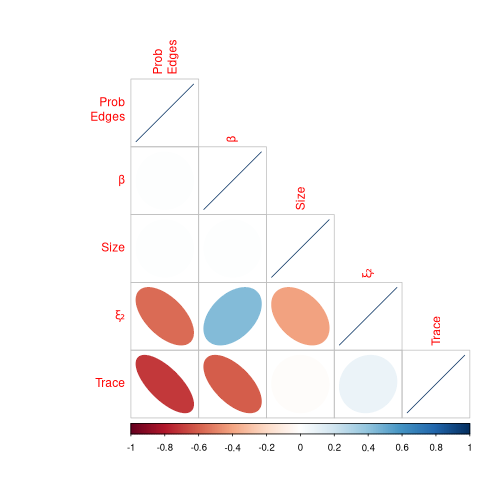
\includegraphics[width=12cm]{media/corrplot.png}
\caption{\label{fig:corrplot}Correlation plot of parameters of \emph{Power Walk} parameters and graph properties.}
\end{figure}

The correlation plot shows a moderate relationship between size, the uniform probability of linking two nodes (\(p\)) and the size of the graph with \(\xi_{2}\). It's worth noting that \(p = \mathrm{mean}\left(\mathbf{A}\right)\).

To inspect these relationships more closely a scatterplot matrix was produced in
figure \ref{plotly_dens} and shown in figure \ref{fig:plotly_dens}. The matrix indicates a
negative relationship between \(\xi_{2}\) with \(p\) and size and a positive
relationship between \(\beta\) and \(\xi_{2}\), these relationships also indicate some degree of interaction.


There also appears to be some relationship between \(\beta\) and the trace of the matrix, this won't be considered for the moment because the trace is not a parameter of the power walk method.

\begin{listing}[htbp]
\begin{minted}[]{r}
plot(data, labels = c("Mean\nEdges", "β", "Size", "ξ₂", "Trace"))
\end{minted}
\caption{\label{plotly_dens}Density of Plot or something, see \ref{fig:plotly_dens}}
\end{listing}


\begin{figure}[htbp]
\centering
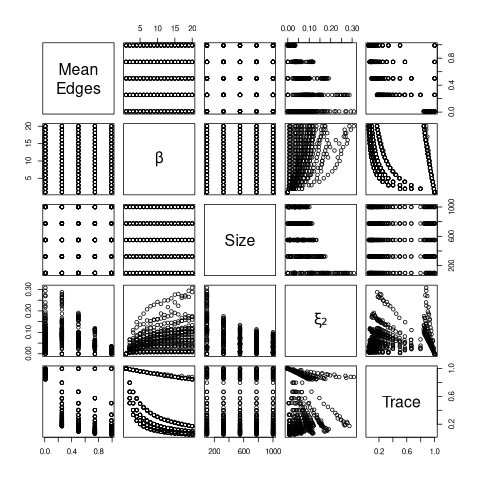
\includegraphics[width=12cm]{media/cor_matrix-er.png}
\caption{\label{fig:plotly_dens}Plot of the Density of the Adjacency Matrix, Beta Value of the Power Walk method with \(\xi_{2}\) represented by the vertical \(z\) axis.}
\end{figure}


By looking at the \(\xi_{2}\) value for a variety of \(p\) values with a
constant size a pattern may be emerge, a corresponding data set is produced in
\ref{er_constant_size}, a plot produced in listing \ref{l:fig:er_constant_size} and the
corresponding plot shown in figure \ref{constant_size_erdos_density}.

\begin{listing}[htbp]
\begin{minted}[]{r}
filename <- "resources/erdosData_constant_size.rds"

if (file.exists(filename)) {
    data2 <- readRDS(filename)
} else {
    p    <- seq(from = 0.01, to = 0.5, length.out = 5   )
    beta <- seq(from = 1  , to = 10  , length.out = 1000)
    size <- 1000

    data2 <- sim_graphs(filename, p, beta, size)
}
\end{minted}
\caption{\label{er_constant_size}Produce a data frame of graphs corresponding to a constant size and link density.}
\end{listing}

\begin{listing}[htbp]
\begin{minted}[]{r}
ggplot(data2, mapping = aes(col = factor(p), x = beta, y = eigenvalue2)) +
  geom_point(size = 0.5) +
  stat_smooth() +
  scale_size_continuous(range = c(0.1,1)) +
  labs(x = "Beta", y = TeX("Second Eigenvalue"), title = TeX("Second Eigenvalue given Matrix Density for 100 vertices") ) +
  guides(col = guide_legend("Link Density"))  +
  theme_bw()
\end{minted}
\caption{\label{l:fig:er_constant_size}Produce a plot of \(\xi_{2}\) for a constant size and a few link densities.}
\end{listing}

\begin{center}
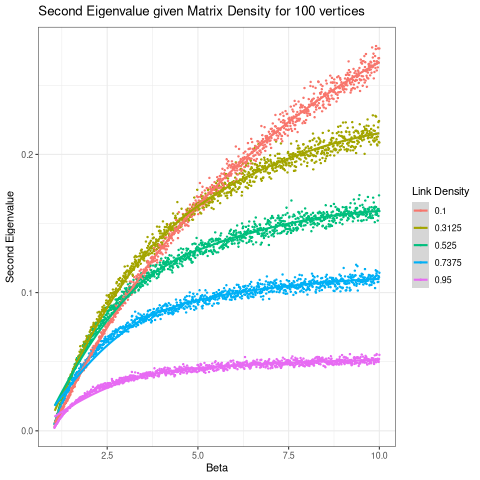
\includegraphics[width=.9\linewidth]{media/constant_size_erdos_density.png}
\end{center}

\begin{figure}[htbp]
\centering
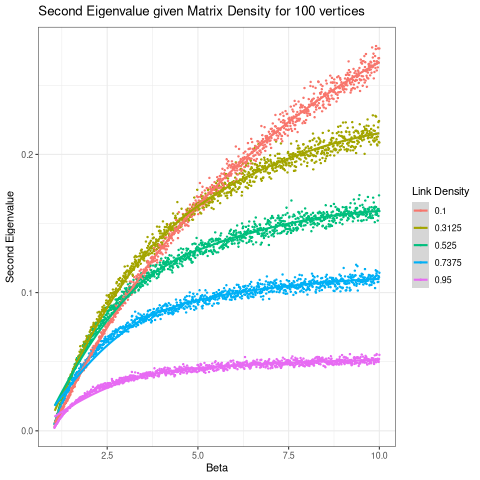
\includegraphics[width=12cm]{media/constant_size_erdos_density.png}
\caption{\label{constant_size_erdos_density}Constant Size Erdos Density}
\end{figure}

This resulting trens are well defined and positive, the data appears to have a
concave down curvature and non constant variance, a sqrt transform is applied in
listing \ref{constant_size_erdos_density_sqrt} and shown in figure .


\begin{listing}[htbp]
\begin{minted}[]{r}
ggplot(data2[30:nrow(data2),], mapping = aes(col = factor(p), x = sqrt(beta), y = eigenvalue2)) +
  geom_point(size = 0.5) +
  stat_smooth() +
  scale_size_continuous(range = c(0.1,1)) +
  labs(x = "sqrt(β)", y = TeX("Second Eigenvalue"), title = TeX("Second Eigenvalue given Matrix Density for 100 vertices") ) +
  guides(col = guide_legend("Link Density"))  +
  theme_bw()
\end{minted}
\caption{\label{constant_size_erdos_density_sqrt}listing:constant\textsubscript{size}\textsubscript{erdos}\textsubscript{density}\textsubscript{sqrt}}
\end{listing}


\begin{figure}[htbp]
\centering
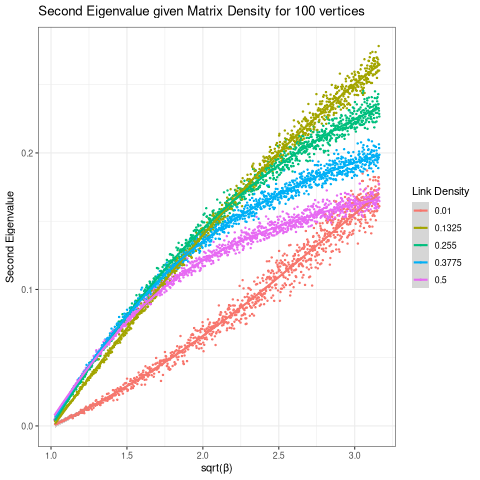
\includegraphics[width=12cm]{media/constant_size_erdos_density_sqrt.png}
\caption{\label{fig:constant_size_erdos_density_sqrt}fig:constant\textsubscript{size}\textsubscript{erdos}\textsubscript{density}\textsubscript{sqrt}}
\end{figure}


The root transform did not significantly normalise the variance or make the
relationship much more linear. The noise would result from using \(p\) as a
probability in forming the graphs as opposed to strictly enforcing the link
density, this variance should be constant so this transform is not desirable.

Both plots in figures
\ref{fig:constant_size_erdos_density_sqrt}
\ref{constant_size_erdos_density}
appear to indicate a more linear relationship between \(\xi_{2}\) and \(\beta\) for smaller link densities and \(\beta\) values.


In order to determine whether or not this relationship persists over many sizes a data set containing the relationship between \(\xi_{2}\) and \(\beta\) was produced for sizes ranging from 100 to 1000 vertices in listing \ref{l:gen_erdos_data_constant_dens}, a corresponding plot was produced in listing \ref{constant_dens_erdos_density} and shown in figure \ref{fig:constant_dens_erdos_density}.


\begin{listing}[htbp]
\begin{minted}[]{r}
filename <- "resources/erdosData_constant_dens.rds"

if (file.exists(filename)) {
    data2 <- readRDS(filename)
} else {
    p    <- 5/100
    beta <- seq(from = 1  , to = 10  , length.out = 1000)
    size <- seq(from = 100, to = 1000, length.out = 5   )

    data2 <- sim_graphs(filename, p, beta, size)
}
\end{minted}
\caption{\label{l:gen_erdos_data_constant_dens}Produce a data set of a variety of sizes ranging from 100 to 1000 vertices.}
\end{listing}

\begin{listing}[htbp]
\begin{minted}[]{r}
ggplot(data2, mapping = aes(col = factor(size), x = (beta), y = eigenvalue2)) +
  geom_point(size = 0.5) +
  stat_smooth() +
  scale_size_continuous(range = c(0.1,1)) +
  labs(x = "β", y = TeX("Second Eigenvalue"), title = TeX("Second Eigenvalue for uniform degree"), subtitle = "mean degree ÷ size = 5%" ) +
  guides(col = guide_legend("Size"))  +
  theme_bw()
\end{minted}
\caption{\label{constant_dens_erdos_density}listing:constant\textsubscript{size}\textsubscript{erdos}\textsubscript{density}}
\end{listing}


\begin{figure}[htbp]
\centering
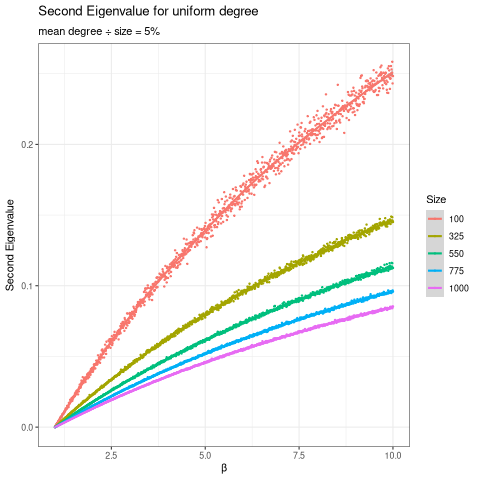
\includegraphics[width=12cm]{media/constant_dens_erdos_density.png}
\caption{\label{fig:constant_dens_erdos_density}fig:constant\textsubscript{dens}\textsubscript{erdos}\textsubscript{density}}
\end{figure}

This relationship appears to have a slight curvature, this curvature is very slight so a root transform is more appropriate than a log transofrm, this is implemented in listing \ref{l:constant_dens_erdos_density_sqrt}  and shown in \ref{fig:constant_dens_erdos_density_sqrt}.

\begin{listing}[htbp]
\begin{minted}[]{r}
ggplot(data2, mapping = aes(col = factor(size), x = sqrt(beta), y = eigenvalue2)) +
  geom_point(size = 0.5) +
  stat_smooth() +
  scale_size_continuous(range = c(0.1,1)) +
  labs(x = TeX("\\sqrt{β}"), y = TeX("Second Eigenvalue"), title = TeX("Second Eigenvalue for uniform degree"), subtitle = "mean degree ÷ size = 5%" ) +
  guides(col = guide_legend("Size"))  +
  theme_bw()
\end{minted}
\caption{\label{l:constant_dens_erdos_density_sqrt}listing:constant\textsubscript{size}\textsubscript{erdos}\textsubscript{density}\textsubscript{sqrt}}
\end{listing}



\begin{figure}[htbp]
\centering
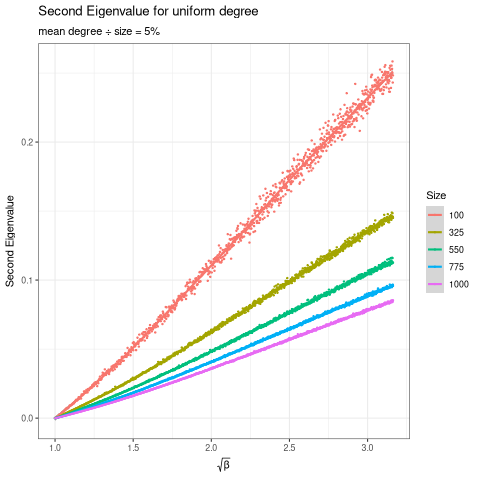
\includegraphics[width=12cm]{media/constant_dens_erdos_density_sqrt.png}
\caption{\label{fig:constant_dens_erdos_density_sqrt}fig:constant\textsubscript{dens}\textsubscript{erdos}\textsubscript{density}\textsubscript{sqrt}}
\end{figure}


The plot shown in \ref{fig:constant_dens_erdos_density_sqrt}  demonstrates a very strong linear relationship between \(\xi_{2}\) and \(\sqrt{\beta}\) for a variety of constant link densities, the variance however is still non-constant over \(\sqrt{\beta}\).

\section{Barabasi Albert Graphs}
\label{barabassi-albert}
\subsection{Theory}
\label{sec:org295fb32}

The \emph{Erdos Renyi} game is a random network, a superior approach to model the web
is to use a scale free networks \cite{barabasiPhysicsWeb2001} such as the
Barabasi-Albert graph \cite{barabasiScalefreeCharacteristicsRandom2000}

The Erdos Renyi game assumes that the number of nodes is constant from beginning
to end, clearly this is not true for networks such as the web. Consider a graph
constructed node by node where each time a new node is introduced it is randomly
connected to another with a constant probability. Despite the probability of
connecting to any given node being constant as in the Erdos Renyi game, such a
graph will favour nodes introduced earlier with respect to the number edges.
This shows that the precense of network growth is an import feature in modelling
networks.

Simply considering growth however is not sufficient to simulate graphs with a
degree distribution consistent with the web
\cite[Ch. 7]{zengPracticalSimulationMethod2013} (see figure ).

When introducing a new node, the probability of linking to any other node is not
uniformly random. When adding links to from one node to another it would be
expected that links to more popular websited would be made (for example if
somebody added a link to a personal website they might be more likely to link to
\emph{Wikipedia} than to the \emph{Encyclopedia of Britannica} simply because it is more
common). A simple approach is to presume that the probability of linking from
one node to another is proportional to the number of links, i.e. a node with
twice as many links will be twice as likely to receive a link from a new node.

These two distinguishing features departing from the \emph{Erdos Renyi} model, known as \emph{Growth} and \emph{Preferrential Attachment}, are what set the Barabassi-Albert model apart from the Erdos-Renyi model and why it is better suited to modelling networks such as the web. \cite[Ch. 7]{barabasiLinkedNewScience2002}


A graph of the internet is \emph{scale free}, this means that the number of nodes of
a graph (\(n\)), having \(k\) edges is given by
 \cite[\textsection 10.7.2]{langvilleGooglePageRankScience2012}:

\begin{align}
n \propto k^{-\gamma}, \quad \exists k \in \mathbb{R}
\end{align}

The Barabassi Albert model implements this scale free approach and predicts that \(\gamma\) values of 3 would fit the model, although, in practice values of in = 2.1 and out = 2.45 are observed. This value would be independent of m. also predicts that \(A \propto m^{2}\): \cite{barabasiScalefreeCharacteristicsRandom2000}

\[
\mathrm{P}\left(k\) \propto m^2 k^{-\gamma}
\]

A practical Simulation method for social networks simulate social network links,
one possibility is \href{https://crpit.scem.westernsydney.edu.au/confpapers/CRPITV144Zeng.pdf}{this paper } \cite{zengPracticalSimulationMethod2013}.

Actually there is a data set available
 \cite{garritanoWikipediaArticleNetworks2019}, I should just analyse that, see \href{file:///home/ryan/Dropbox/DataSci/Visual\_Analytics/Assessment/the-marvel-universe-social-network/plotly3d\_Marvel.r}{how
it was done in Visual Analytics as a reminder}.



\begin{listing}[htbp]
\begin{minted}[]{r}
layout(matrix(1:2, nrow = 2))
col  <- "Mediumpurple"
n <- 1000
hist(
  igraph::degree(igraph::sample_pa(n, 0.2)),
  binwidth = 0.3,
  xlab = "",
  main = "Barabassi-Albert Degree Distribution",
  col = col, freq = FALSE
)

hist(igraph::degree(igraph::erdos.renyi.game(n, 0.2)),
     main= "Erdos-Renyi Degree Distribution",
     col = col,
     binwidth = 0.3,
     xlab = "",
     freq = FALSE )
\end{minted}
\caption{\label{degree-distribution-hist}Simulate Erdos-Renyi and Barabassi-Albert graphs in order to measure the degree distribution,  shown in \ref{fig:degree-distribution-hist}}
\end{listing}


\begin{figure}[htbp]
\centering
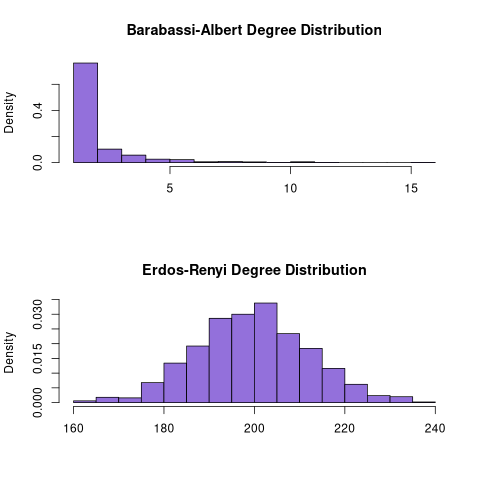
\includegraphics[width=12cm]{media/degree_dist_er_ba.png}
\caption{\label{fig:degree-distribution-hist}histograms of degree distribution of Erdos-Renyi and Barabassi-Albert graphs produced in listing \ref{degree-distribution-hist}}
\end{figure}

\subsection{Modelling}
\label{sec:orgb52cc3e}
At each step of the Barabassi-Albert algorithm, one node is added and linked to \(m\) other nodes with a probability proportional to the degree of that vertex.

This means that the average of the unweighted adjacency matrix would be given by \(p = \mathrm{mean}\left(\mathbf{A}\right) \in \left[ \frac{m}{n}, \frac{m+1}{n} \right]\) and the relationship identified in \ref{erdos-renyi} can be determined from the parameters of a scale-free network.

In practice though measuring \(m\) (as the mean out degree) will be imprecise and the adjacency matrix will be wieghted any way, so taking the mean of the weighted adjacency matrix would still be necessary to implement this type of model in practice.

A function to generate a random Barabassi-Albert graph and return the value of
\(\xi_{2}\) corresponding to the Power Walk method is provided in listing
\ref{random_graph_pa}, another function to map this over the cartesian product of
input variables is provided in listing \ref{sim_graphs_pa} and finally a dataset containing 9
different link densities was created in listing \ref{l:gen_ba_data}.

This data plotted by listing \ref{l:ba_data_plot} and shown in \ref{fig:ba_data_plot}.

\begin{listing}[htbp]
\begin{minted}[]{r}
random_graph_pa <- function(m, beta, size) {
      g1 <- igraph::sample_pa(n = size, power = 3, m = m)
      A <- igraph::get.adjacency(g1) # Row to column
      A <- Matrix::t(A)

#      A_dens <- mean(A)
      T      <- PageRank::power_walk_prob_trans(A, beta = beta)
      tr     <- sum(diag(T))
      e2     <- eigen(T, only.values = TRUE)$values[2] # R orders by descending magnitude
      return(c(abs(e2), tr))
}
\end{minted}
\caption{\label{random_graph_pa}A function to build a random graph using the Barabassi-Albert Model and return the value of \(\xi_{2}\) corresponding to the \emph{Power Walk} method.}
\end{listing}

\begin{listing}[htbp]
\begin{minted}[]{r}
sim_graphs_pa <- function(filename, m, beta, size) {

    input_var <- expand.grid("m" = m, "beta" = beta, "size" = size)

    nc <- length(random_graph_pa(1, 1, 1))
    Y  <- matrix(ncol = nc, nrow = nrow(input_var))
    for (i in 1:nrow(input_var)) {
        X     <- as.vector(input_var[i,])
        Y[i,] <-  random_graph_pa(X$m, X$beta, X$size)
        print(i/nrow(input_var))
    }
    if (sum(abs(Y) != abs(Re(Y))) == 0) {
        Y <- Re(Y)
    }
    Y <- as.data.frame(Y); colnames(Y) <- c("eigenvalue2", "trace")
    data2 <- cbind(input_var, Y)
    saveRDS(data2, filename)
    return(data2)
}
\end{minted}
\caption{\label{sim_graphs_pa}Return \(\xi_{2}\) values by mapping the \texttt{random\_graph\_pa} function from listing \ref{random_graph_pa} over the cartesian product of input variables.}
\end{listing}


\begin{listing}[htbp]
\begin{minted}[]{r}
filename <- "resources/BAData.rds"

if (file.exists(filename)) {
    data2 <- readRDS(filename)
} else {
    m    <- seq(from = 1, to = 9, length.out = 3)
    beta <- seq(from = 1, to = 6, length.out = 30)
    sz   <- seq(from = 100, to = 500, length.out = 3) %>% rev() # Big numbers first

    input_var <- expand.grid("m" = m, "beta" = beta, "size" = sz)

    data2 <- sim_graphs_pa(filename, p, beta, size)
}
\end{minted}
\label{l:gen_ba_data}
\end{listing}

\begin{listing}[htbp]
\begin{minted}[]{r}
data2$p <- round((data2$m/data2$size), 2)

ggplot(data2, mapping = aes(col = factor(p), x = beta, y = eigenvalue2)) +
  geom_point(size = 0.5) +
  stat_smooth(method = 'lm', size = 0.4) +
  scale_size_continuous(range = c(0.1,1)) +
  labs(x = "Beta", y = TeX("Second Eigenvalue"), title = TeX("Second Eigenvalue given Matrix Density") ) +
  guides(col = guide_legend("Link Density (by m/n)"))  +
  theme_bw()
\end{minted}
\caption{\label{l:ba_data_plot}l:ba\textsubscript{data}\textsubscript{plot}}
\end{listing}


\begin{figure}[htbp]
\centering
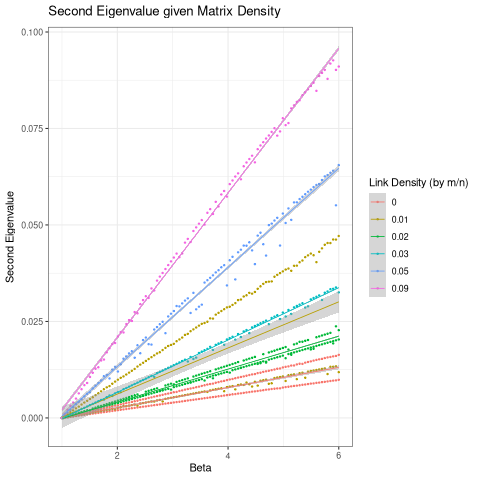
\includegraphics[width=12cm]{media/constant_dens_ba_density_sqrt.png}
\caption{\label{fig:ba_data_plot}fig:ba\textsubscript{data}\textsubscript{plot}}
\end{figure}

Due to the relationship between size and density in the barabassi albert model this approach seems to work even better for BA graphs, which is precisely the type of graph where we might anticipate the use of the power walk method.

The low link densities are such that there is no need for a log/root transform either, such a transform was found to be unsuitable in \S \ref{correlation-plot} so this is encouraging.

To determine the relationship that the link density \(p\) may have, the value of
\(\beta\) will be fixed and the behaviour of \(\xi_{2} \sim p\) can be
investigated. A corresponding data set is produced in listing
\ref{l:baData_constant_size}, plotted in listing \ref{l:ba_data_constant_size_plot} and
shown in figure \ref{fig:ba_data_constant_size_plot}.



\begin{listing}[htbp]
\begin{minted}[]{r}
filename <- "resources/BAData_constant_size.rds"

if (file.exists(filename)) {
    data2 <- readRDS(filename)
} else {
    m       <- seq(from = 1, to = 9, length.out = 15)
    beta    <- 5
    size    <- seq(from = 100, to = 500, length.out = 7)

    data2 <- sim_graphs_pa(filename, m, beta, size)
}
\end{minted}
\caption{\label{l:baData_constant_size}l:baData\textsubscript{constant}\textsubscript{size}}
\end{listing}

\begin{listing}[htbp]
\begin{minted}[]{r}
data2$p <- round((data2$m/data2$size), 2)

names(data2)
ggplot(data2, mapping = aes(col = factor(round(size)), x = p, y = eigenvalue2)) +
  geom_point(size = 0.5) +
  stat_smooth(method = 'lm', size = 0.4, se = FALSE) +
  scale_size_continuous(range = c(0.1,1)) +
  labs(x = "p", y = TeX("Second Eigenvalue"), title = TeX("Second Eigenvalue given Matrix Density") ) +
  guides(col = guide_legend("Size"))  +
  theme_bw()
\end{minted}
\caption{\label{l:ba_data_constant_size_plot}l:ba\textsubscript{data}\textsubscript{constant}\textsubscript{size}\textsubscript{plot}}
\end{listing}


\begin{figure}[htbp]
\centering
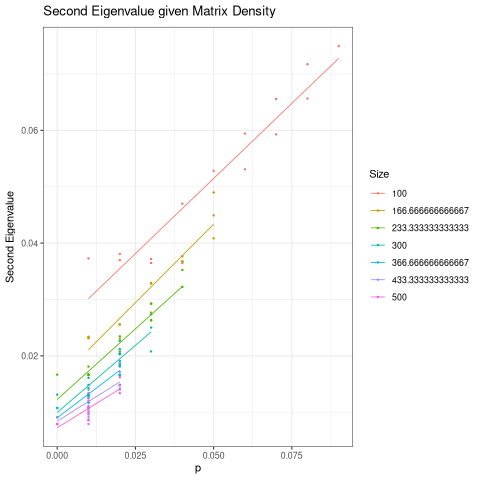
\includegraphics[width=12cm]{media/ba_constant_size_plot.png}
\caption{\label{fig:ba_data_constant_size_plot}fig:ba\textsubscript{data}\textsubscript{constant}\textsubscript{size}\textsubscript{plot}}
\end{figure}


This seems to suggest that the effect on the eigenvalue that \(p\) has depends on the size of the graph, so  \(p\) and size interact with respect to \(\xi_{2}\).

Hence an appropriate model will consider the value of \(p\), \(p*n\) and \(\beta\), where \(n\) is the size of the graph.

\subsubsection{Model}
\label{sec:org767df9c}
A simple model to consider the variables found to influence \(\xi_{2}\) is
multiple linear regression, although it is a very simple model it is easy to
interpret and may offer insights into the behaviour of \(\xi_{2}\) in response
to different graphs.

More data was generated and a model fitted to training data in listing
\ref{l:mlm_hist_ba} a corresponding residual histogram for the testing data is provided in \ref{fig:mlm_hist_ba} and a summary of the model provided in listing \ref{mod_summary}.

In fitting the model in listing \ref{l:mlm_hist_ba} the identity \(p = \frac{m}{n}\) was implemented because taking the mean value of a large matrix is resource intensive and would have reduced the number of data points in the analysis.


\begin{listing}[htbp]
\begin{minted}[]{r}
filename <- "resources/BAData_lots.rds"

# Load the DAta
if (file.exists(filename)) {
    data_lots <- readRDS(filename)
} else {
    m       <- seq(from = 1, to = 9, length.out = 10)
    beta    <- seq(from = 1, to = 20, length.out = 40)
    size    <- seq(from = 100, to = 500, length.out = 5) %>% rev()
    size    <- c(size, 750, 1000)

    data_lots <- sim_graphs_pa(filename, m, beta, size)
}

# Create the link density variable
data2   <- data_lots
data2$p <- data2$m/data2$size

# Use 80% testing data
n   <- nrow(data2)
r   <- 0.8
train <- sample(x = 1:nrow(data2), size = r*n)

# Fit the Model
mod       <- lm(eigenvalue2 ~ 0 + p*size + p + beta, data = data2, subset = train)
test_pred <- predict(object = mod)[-train]
test_res  <- test_pred-data2$eigenvalue2[-train]

# Make the Plot
q <- quantile(test_res, c(0.025, 0.5, 0.975))
quantile(test_res)
cil <- q[1]
cih <- q[2]
cir <- q[3]

hist(test_res, breaks = 50, xlab = "Residuals",
     main = "Histogram of Residuals")
abline(v = c(cil, cih, cir))

\end{minted}
\caption{\label{l:mlm_hist_ba}l:mlm\textsubscript{hist}\textsubscript{ba}}
\end{listing}

\begin{figure}[htbp]
\centering
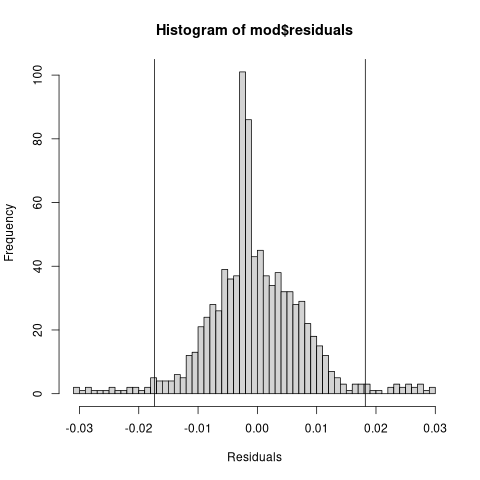
\includegraphics[width=12cm]{media/ba_hist_mlm_mod.png}
\caption{\label{fig:mlm_hist_ba}Histogram of the test set residuals for the multiple linear regression model fitted in listing \ref{l:mlm_hist_ba}, these residuals appear reasonably normal and are centred around zero, this suggests that the model may be an appropriate estimate on the domain that it was fitted.}
\end{figure}


\begin{listing}[htbp]
\begin{minted}[]{r}
summary(mod)
\end{minted}
\caption{\label{mod_summary}Summarise the Coefficients of the model.}
\end{listing}

\begin{verbatim}

Call:
lm(formula = eigenvalue2 ~ 0 + p * size + p + beta, data = data2)

Residuals:
      Min        1Q    Median        3Q       Max
-0.108811 -0.009673 -0.001948  0.007289  0.069467

Coefficients:
         Estimate Std. Error t value Pr(>|t|)
p       1.348e+00  2.661e-02  50.651   <2e-16 ***
size   -3.404e-05  1.292e-06 -26.358   <2e-16 ***
beta    3.923e-03  5.205e-05  75.367   <2e-16 ***
p:size -1.446e-03  1.683e-04  -8.592   <2e-16 ***
---
Signif. codes:  0 ‘***’ 0.001 ‘**’ 0.01 ‘*’ 0.05 ‘.’ 0.1 ‘ ’ 1

Residual standard error: 0.01805 on 2796 degrees of freedom
Multiple R-squared:  0.9089,	Adjusted R-squared:  0.9088
F-statistic:  6975 on 4 and 2796 DF,  p-value: < 2.2e-16
\end{verbatim}

The residuals appear reasonably normal, this suggests that the model may be an appropriate estimation over the domain on which it was fitted, the corresponding model is given by:

\begin{align}
\left\lvert \xi_{2} \right\rvert &= 1.34 p -  \frac{3.4n}{10^{5}} + \frac{3.9\beta}{10^{3}} - \frac{1.4 p n}{10^{3}} \\
        &p = \mathrm{mean}\left( \mathbf{A}\right)
\end{align}

For an unweighted adjacency matrix from the internet we may expect:

\begin{align}
p &\approx \frac{m}{n} \\
  &= \frac{\mathrm{mean}\left(\mathrm{outdegree}\right)}{n}
\end{align}

for larger scale free graphs \(p \rightarrow 0\) so this model seems to suggest that the eigenvalue will be reduced for larger graphs.

To test the model, we can measure the eigenvalue resulting from values within the domain of the model and from outside the domain:

\begin{minted}[]{r}
m         <- 1
beta      <- 3
size <- n <- 50


g <- igraph::sample_pa(power = 3, n = n, m = m)
A <- t(as.matrix(igraph::get.adjacency(g)))
W <- PageRank::power_walk_prob_trans(A, beta = beta)

p <- mean(A)
(e2 <- abs(eigen(W, only.values = TRUE)$values[2]) )

abs(e2_pred <-
  p      *   1.344
+ size   * - 3.393e-05
+ beta   *   3.918e-03
+ p*size * - 1.437e-03
  )
\end{minted}

\begin{verbatim}
[1] 0.03689031
[1] 0.03499164
\end{verbatim}


That's actually pretty close, but, how does it perform on graphs outside the range of size?

\begin{minted}[]{r}
m         <- 1
beta      <- 3
size <- n <- 2000


g <- igraph::sample_pa(power = 3, n = n, m = m)
A <- t(as.matrix(igraph::get.adjacency(g)))
W <- PageRank::power_walk_prob_trans(A, beta = beta)

p <- mean(A)
(e2 <- abs(eigen(W, only.values = TRUE)$values[2]) )

abs(e2_pred <-
  p      *   1.344
+ size   * - 3.393e-05
+ beta   *   3.918e-03
+ p*size * - 1.437e-03
  )
\end{minted}

\begin{verbatim}
[1] 0.001329781
[1] 0.03968164
\end{verbatim}


Unfourtunately this suggests that for large graphs this model is not a good fit,
which means that this model can only provide insight into the behaviour of
\(\xi_{2}\) for graphs with less than 1000 vertices.

\section{Relating the Power Walk to the Random Surfer}
\label{relate-to-random-surfer}
It has been shown that \(\xi_{2} \leq \alpha\) for a transition probability matrix corresponding the random surfer model and that \(\xi_{2} = \alpha\) if there are atleast two closed subgraphs in the initial network \cite{haveliwalaSecondEigenvalueGoogle2003}. This is demonstrated by figure \ref{example-rs-graph} and figure \ref{r-var-random-surfer} where \(\alpha = \xi_{2} = 0.8123456789\).

Finding a connection between the random surfer and the the power walk methods could provide insight into the relationship of \(\xi_{2}\) and the parameters of the power walk method.

\subsection{Introduction}
\label{sec:org07b66b7}
Consider the equation:


\begin{align*}
\mathbf{T}&= \mathbf{B}\mathbf{D}_{\mathbf{B}}^{- 1} \\
&= \left( \mathbf{B}+  \mathbf{O} - \mathbf{O} \right) \mathbf{D}_{\mathbf{B}}^{- 1} \\
\end{align*}


Break this into to terms so that we can simplify it a bit:


\begin{align*}
    \mathbf{T} &= \Bigg[ \left( \mathbf{B}- \mathbf{O} \right)\mathbf{D}_{\mathbf{B}}^{- 1} \Bigg] + \Bigg\{  \mathbf{O}\mathbf{D}_{\mathbf{B}}^{- 1} \Bigg\}
\end{align*}
\subsection{Value of [1st Term]}
\label{value-of-1st-term}
Observe that for all \(\forall i,j\in \mathbb{Z}^+\):


\begin{align*}
\mathbf{A}_{i, j} \in \left\{0, 1\right\} \\
\implies  \mathbf{B}^{\mathbf{A}_{i, j}} &\in \left\{\beta^0, \beta^1\right\} \\
                     &= \left\{1, \beta \right\}  \\
                      \implies  \beta \mathbf{A} = \left\{1, \beta \right\}
\end{align*}


Using this property we get the following


\begin{align*}
\mathbf{B}_{i,j}- \mathbf{O}_{i,j} = \left( \beta^{\mathbf{A}_{i,j}} -1 \right) &=
\begin{cases}
    0      , &\enspace \mathbf{A}_{i,j}=0  \\
    \beta-1, &\enspace \mathbf{A}_{i,j}=1  \\
\end{cases} \\
\left( \beta- 1 \right) \mathbf{A}_{i,j} &=
\begin{cases}
    0      , &\enspace \mathbf{A}_{i,j}=0  \\
    \beta-1, &\enspace \mathbf{A}_{i,j}=1  \\
\end{cases} \\
\end{align*}


This means we have


\begin{align*}
\mathbf{A} \in \left\{0, 1\right\} \forall i,j  \implies   \mathbf{B}_{i,j}- \mathbf{O}_{i,j} &= \left( \beta-1 \right) \mathbf{A}_{i,j}
\end{align*}



\begin{align*}
\mathbf{B}&= \left( \mathbf{B}+  \mathbf{O}- \mathbf{O} \right) \\
&= \left( \mathbf{B}- 1 \right)
\end{align*}

\subsection{Value of \{2nd Term\}}
\label{value-of-2nd-term}
\begin{align*}
\mathbf{O} \mathbf{D_B^{- 1}} &=
\begin{pmatrix}
    1 & 1      & 1 &        \\
    1 & 1      & 1 &\cdots  \\
    1 & 1      & 1 &        \\
      & \vdots &   &\ddots
\end{pmatrix}
\begin{pmatrix}
    \frac{1}{\delta_1} & 1                    & 1                   & \\
    1                  & \frac{1}{\delta_{2}} & 1 \cdots            & \\
    1                  & 1                    &  \frac{1}{\delta_3} & \\
               & \vdots &             &                     \ddots
\end{pmatrix}
\\
&= n
\begin{pmatrix}
    \frac{1}{n} & \frac{1}{n}      & \frac{1}{n} &        \\
    \frac{1}{n} & \frac{1}{n}      & \frac{1}{n} &\cdots  \\
    \frac{1}{n} & \frac{1}{n}      & \frac{1}{n} &        \\
      & \vdots &   &\ddots
\end{pmatrix}
\begin{pmatrix}
    \frac{1}{\delta_1} & 1                    & 1                   &        \\
    1                  & \frac{1}{\delta_2}    & 1                   & \cdots \\
    1                  & 1                    &  \frac{1}{\delta_3} &        \\
                       & \vdots               &                     & \ddots
\end{pmatrix}
\\
&= n \mathbf{E}\mathbf{D_B}^{-1}
\end{align*}


where the following definitions hold (\(\forall i, j \in \mathbb{Z}^+\)):

\begin{itemize}
\item \(\mathbf{E}_{i, j} = \frac{1}{n}\)
\item \(\mathbf{D_B}^{-1}_{k, k} = \frac{1}{\delta_k}\)
\item The value of \(\delta\) is value that each term in a column must be
divided by to become zero, in the case of the power walk that is just
\(\frac{1}{\mathtt{colSums}\left( \mathbf{B} \right)} = \vec{1}\mathbf{B}\),
but if there were zeros in a column, it would be necessary to swap out
the \$0\$s for \$1\$s and then sum in order to prevent a division by zero
issue and because the 0s should be left.
\item \(\mathbf{A}\in \left\{0, 1\right\} \forall i,j\) is the unweighted
adjacency matrix of the relevant graph.
\end{itemize}

putting this all together we can do the following:


\begin{align*}
\mathbf{T}&= \mathbf{B}\mathbf{D}^{- 1}_{\mathbf{B}} \\
&= \left( \mathbf{B}+  \mathbf{O} - \mathbf{O} \right) \mathbf{D}_{\mathbf{B}}^{- 1} \\
&= \left( \mathbf{B}- \mathbf{O} \right)\mathbf{D}_{B}^{- 1}  +  \mathbf{O} {\mathbf{D}_{\mathbf{B}}^{- 1}} \\
 \intertext{From above:} \\
&= \left( \beta- 1 \right) \mathbf{A}_{i,j} +  n \mathbf{E} \mathbf{D}_{\mathbf{B}}^{- 1}\\
&= \mathbf{A}_{i,j}\left( \beta- 1 \right)  +  n \mathbf{E} \mathbf{D}_{\mathbf{B}}^{- 1}\\
 \intertext{because $\mathbf{D} \mathbf{D}^{- 1} = \mathbf{I}$ we can multiply one side through:} \\
&= \mathbf{D}_{\mathbf{A}} \mathbf{D}_{\mathbf{A}}^{- 1}\mathbf{A}_{i,j}\left( \beta- 1 \right)  +  n \mathbf{E} \mathbf{D}_{\mathbf{B}}^{- 1}\\
\end{align*}


But the next step requires showing that:


\begin{align*}
\left( \beta-1 \right)\mathbf{D}_\mathbf{A} \mathbf{D}_{\mathbf{B}}^{- 1} &= \mathbf{I} - n \mathbf{D}_{B}^{- 1}
\end{align*}

\subsection{Equate the Power Walk to the Random Surfer}
\label{sec:orge516de9}
Define the matrix \(\mathbf{D}_{\mathbf{M}}\):

\begin{align}
    \mathbf{D}_{\mathbf{M}} = \mathrm{diag}\left( \mathtt{colSum} \left( \mathbf{M} \right) \right) &= \mathrm{diag} \left( \vec{1} \mathbf{M} \right)
\end{align}


To scale each column of that matrix to 1, each column will need to be divieded by the column sum, unless the column is already zero, this needs to be done to turn an adjacency matrix into a transition probability matrix:

\begin{align}
    \mathbf{D}_{\mathbf{A}} ^{- 1} :  \left[     \mathbf{D}_{\mathbf{A}} ^{- 1}  \right]_i =
    \begin{cases}
	0 ,& \quad \left[ \mathbf{D}_{\mathbf{A}} \right]_i = 0 \\
	\left[ \frac{1}{\mathbf{D}_{\mathbf{A}}} \right] ,& \enspace \enspace \left[ \mathbf{D}_{\mathbf{A}} \right]_i \neq 0
    \end{cases}
\end{align}

In the case of the power walk \(\mathbf{B}= \beta^{\mathbf{A}} \neq 0\) so it is sufficient:

\begin{align}
    \mathbf{D}_{\mathbf{B}}^{- 1} &= \frac{1}{\mathrm{diag}\left( \vec{1} \left(\mathbf{\beta^{\mathbf{A}}  \right) } \right)}
\end{align}


Recall that the \emph{power walk} gives a transition probability matrix:

\begin{align}
%    \mathbf{T} &= \mathbf{a} \text{\fboxsep=.2em\fbox{$x$}} \\
    \text{\textbf{Power Walk}} \nonumber \\
\mathbf{T} &= \text{\fboxsep=.2em\fbox{$\mathbf{A}\mathbf{D}_{\mathbf{A}}^{- 1}$}}  \mathbf{D}_{\mathbf{A}} \left( \beta - 1 \right) \mathbf{D}_{\mathbf{B}}^{- 1} + \text{\fboxsep=.2em\fbox{$\mathbf{E}$}} n \mathbf{D}_{\mathbf{B}}^{- 1}  \label{eq:pwbx}\\
    \text{\textbf{Random Surfer}} \nonumber \\
    \mathbf{T} &= \alpha \text{\fboxsep=.2em\fbox{$\mathbf{A}\mathbf{D}_{\mathbf{A}}^{- 1}$}}  + \left( 1-\alpha \right) \text{\fboxsep=.2em\fbox{$\mathbf{E}$}}
\end{align}

So these are equivalent when:

\begin{align}
\mathbf{D}_{\mathbf{A}}   \left( \beta -  1 \right)\mathbf{D}_{\mathbf{B}^{- 1}} &=\mathbf{I}  \alpha \label{fl} \\
    \ \nonumber \\
  \vec{1}  \left( 1- \alpha \right) &=  - n \mathbf{D}_{\mathbf{B}}^{- 1}  \nonumber \\
    \implies  \vec{1}\alpha &=  \vec{1}- n \mathbf{D}_{\mathbf{B}}^{- 1} \label{st} \\
    \intertext{Hence we have:} \notag \\
\mathbf{D}_{\mathbf{A}}  \left( \beta -  1 \right)\mathbf{D}_{\mathbf{B}}^{- 1} &=  \vec{1}\alpha =  \mathbf{I}- n \mathbf{D}_{\mathbf{B}}^{- 1} \label{eq:eqalpha}
\end{align}

Solving for \(\beta\):

\[
\beta \mathbf{J}  = \left( 1 - \Theta \right) \Theta^{-1} \label{eq:betadef}
\]

where: \footnote{This is similar to a signmoid function, which is a solution to \(p \propto p(1-p)\), I wonder if this provides a connection to the exponential nature of the power walk}

\begin{itemize}
\item \(\Theta = \mathbf{D}_{\mathbf{A}} \mathbf{D}_{\mathbf{B}}^{- 1}\)
\end{itemize}

If \(\beta\) is set accordingly then by \eqref{eq:eqalpha}:

\begin{align}
    \mathbf{A}\left( \beta- 1 \right) \mathbf{D}_{\mathbf{B}}^{- 1} &= \alpha = \mathbf{I}- n \mathbf{D}_{\mathbf{B}}^{- 1} \nonumber \\
     \implies  \mathbf{A}\left( \beta- 1 \right) \mathbf{D}_{\mathbf{B}}^{- 1} &=  \mathbf{I}- n \mathbf{D}_{\mathbf{B}}^{- 1}
\end{align}

And setting \(\Gamma = \mathbf{I}- n \mathbf{D}_{\mathbf{B}}^{- 1}\)  from \eqref{st} and putting in \eqref{eq:pwbx} we have:

\begin{align}
\mathbf{T} &= \text{\fboxsep=.2em\fbox{$\mathbf{A}\mathbf{D}_{\mathbf{A}}^{- 1}$}}  \mathbf{D}_{\mathbf{A}} \left( \beta - 1 \right) \mathbf{D}_{\mathbf{B}}^{- 1} + \text{\fboxsep=.2em\fbox{$\mathbf{E}$}} n \mathbf{D}_{\mathbf{B}}^{- 1}  \nonumber \\
  \mathbf{T} &= \Gamma \text{\fboxsep=.2em\fbox{$\mathbf{A}\mathbf{D}_{\mathbf{A}}^{- 1}$}}  + \left( 1-\Gamma \right) \text{\fboxsep=.2em\fbox{$\mathbf{E}$}} \nonumber \\
  \ \nonumber \\
  \mathbf{T} &= \Gamma \mathbf{A}\mathbf{D}_{\mathbf{A}}^{- 1}  + \left( 1-\Gamma \right) \mathbf{E}
  \end{align}

Where \(\mathbf{E}\) is square matrix of \(\frac{1}{n}\) as in \eqref{eq:bgval1}  \eqref{eq:bgVal2}

\subsection{Conclusion}
\label{sec:orgad79e88}
So when the adjacency matrix is stictly boolean, the power walk is equivalent to the random surfer.

More investigation will be required to determine further connections between these two methods.

\section{Conclusion}
\label{sec:orgc228632}
In this report an approach to implement and investigate the random surfer and random walk \emph{PageRank} methods was presented and a linear model was implemented to try and provide insight into the behaviour of the second eigenvalue of the probability transition matrix corresponding to the power walk method.

The model appears not to perform well for graphs over 1000 vertices, this is unfourtunate and limits the amount of insight the model can provide into the behaviour of the power walk method.

A relationship between the random surfer and power walk method was also presented, this relationship appears to be restricted to unweighted adjacency matrices, it is not clear however if this could be expanded.

Further investigation is required to understand the relationship between the
second eigenvalue and the method parameters of the power walk method, such
further investigation should focus on investigating the relationship between the
power walk and random surfer models and implementing non-linear models.


\section{Appendix}
\label{sec:orgdf858c5}

\begin{listing}[htbp]
\begin{minted}[]{r}
library(Matrix)
library(igraph)
n <- 200
m <- 5
power <- 1
g <- igraph::sample_pa(n = n, power = power, m = m, directed = FALSE)
plot(g)
A <- t(get.adjacency(g))
plot(A)
image(A)


# Create a Plotting Region
par(pty = "s", mai = c(0.1, 0.1, 0.4, 0.1))


# create the image

title=paste0("Undirected Barabassi Albert Graph with parameters:\n Power = ", power, "; size = ", n, "; Edges/step = ", round(m))
image(A, axes = FALSE, frame.plot = TRUE, main = title, xlab = "", ylab = "",  )
\end{minted}
\caption{\label{r-den_undir_ba}\textbf{\emph{R}} code to produce an image illustrating the density of a simulated Barabasi-Albert graph, the \emph{Barabasi-Albert} graph is a good analouge for the link structure of the internet \cite{langvilleGooglePageRankScience2012,barabasiPhysicsWeb2001,barabasiScalefreeCharacteristicsRandom2000} see the output in figure \ref{fig:den_undir_ba}}
\end{listing}

\begin{figure}[htbp]
\centering
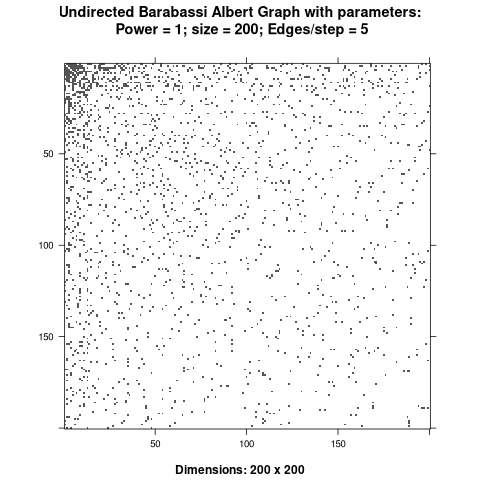
\includegraphics[width=12cm]{media/DensityUndirectedBA.png}
\caption{\label{fig:den_undir_ba}Plot of the adjacency matrix corresponding to a Barabassi-Albert (i.e. \emph{Scale Free}) Graph produced by listing \ref{r-den_undir_ba}, observe the matrix is quite sparse.}
\end{figure}
\subsection{Graph Diagrams}
\label{sec:orgc4aeb84}
Graph Diagrams shown in \ref{markov} where produced using \texttt{DOT} (see \cite{DOTLanguage,DOTGraphDescription2020}).
\section{my to do list}
\label{sec:org7d319ec}
\subsection{Use BA Graphs}
\label{sec:org4d81e01}
\subsection{Look at the ScatterPlot Matrix}
\label{sec:org3ce57e4}
\subsection{Compare eigenvalue2 and iterations}
\label{sec:org318b653}

\subsection{Look at using an SVM/logReg or other classifier}
\label{sec:orgdab29a4}
Use a ROC curve to find which threshold of e2 predicts a below average number of iterations.

Predict that e2 value?
\subsubsection{Measure Iterations and E2 values}
\label{sec:orgdbb675e}
\subsubsection{Are any values indicative of E2 Values?}
\label{sec:orgc50c266}
\subsubsection{Use Method Parameters with a log reg to predict a number of iterations}
\label{sec:orgb67a6ec}
\subsubsection{Use a ROC Curve to set a threshold}
\label{sec:org2ec9276}
\subsubsection{Discuss the results.}
\label{sec:orgd3fd2dd}
\subsection{Tie the Report together.}
\label{sec:org10f5b1d}
\subsection{Typeset the Report}
\label{sec:orgf11c080}

\subsection{TODO Diamater}
\label{sec:orgdc860c9}
Diamater of the web sounds like a fun read \cite{albertDiameterWorldWideWeb1999}
\subsection{Improving the Performance of Page Rank}
\label{sec:orgd337bf5}

This:

\begin{quote}
Another approach involves involves reordering the problem and taking advantage
of the fact that the transition probability matrix is sparse  in order
to produce a new algorithm which cannot perform worse than the \emph{power method}
but has been shown to improve the rate of convergence in certain cases.
\cite{langvilleReorderingPageRankProblem2006}.
\end{quote}


There was also a book that I downloaded that mentioned it

Accellerating the Computatoin of Page Rank \cite{langvilleGooglePageRankScience2012}
\end{document}
